% --------------------------- Implementation ---------------------------------

\section{Implementation}
\subsection{Features From RM}
\noindent
For the initial prototype development, a subset of the requirements from the Requirement Matrix (RM) was carefully selected to focus on implementing core functionalities and demonstrating proof of concept. The selection was based on a combination of high-priority functional requirements that form the backbone of the system, ensuring that critical features are built and validated before expanding the scope.

The requirements chosen for the prototype primarily involve data preprocessing, model training, and evaluation processes. These requirements were selected because they are fundamental to the project's success, ensuring that the data pipeline and model implementation work seamlessly together. This subset of features lays the groundwork for later integration with additional components and more complex functionality.

The filtered part of the RM focuses on the following high-priority requirements: data cleaning and feature extraction, training of machine learning models, and evaluation of model performance using standard metrics. These requirements were identified as crucial because they directly impact the system's ability to handle data, learn patterns, and provide meaningful outputs. Without successfully implementing these core features, the overall effectiveness of the solution would be significantly reduced.

Furthermore, these selected features align with the project’s goals and provide a clear pathway for incremental development. By narrowing down the requirements to these foundational aspects, the development team can ensure that the prototype is not only functional but also extensible, providing a robust framework for future enhancements.

\begin{figure}[h!]  
    \centering
    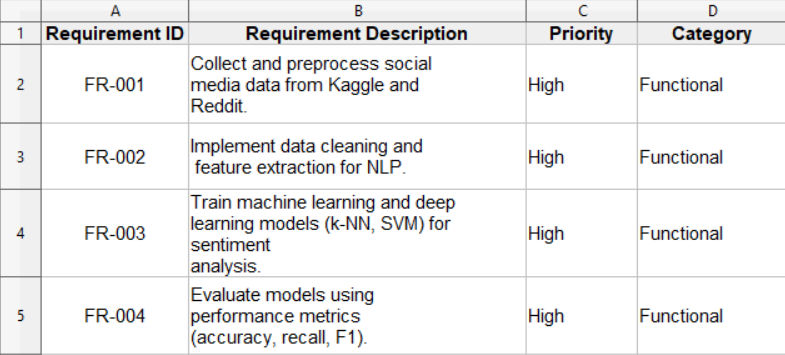
\includegraphics[width=0.85\textwidth]{Images/RM_part_for_implementation.png}  
    \caption{Features from Requirement Matrix}
    \label{Features from Requirement Matrix}  % Label for referencing the figure
\end{figure}

\subsection{Steps of Compilation, Execution and Setup}
\begin{enumerate}
    \item \textbf{Setup the Development Environment}
    \begin{itemize}
        \item Ensure Python 3.x is installed on your system.
        \item Install a virtual environment package if not already available:
        \begin{verbatim}
        pip install virtualenv
        \end{verbatim}
        \item Create a virtual environment for the project:
        \begin{verbatim}
        python -m venv project_env
        \end{verbatim}
        \item Activate the virtual environment:
        \begin{itemize}
            \item For Windows:
            \begin{verbatim}
            .\project_env\Scripts\activate
            \end{verbatim}
            \item For Linux/Mac:
            \begin{verbatim}
            source project_env/bin/activate
            \end{verbatim}
        \end{itemize}
    \end{itemize}

    \item \textbf{Install Required Libraries}
    \begin{itemize}
        \item Install the necessary Python libraries using the following command:
        \begin{verbatim}
        pip install pandas numpy scikit-learn matplotlib
        \end{verbatim}
        \item If your project has additional dependencies, include them as well:
        \begin{verbatim}
        pip install tensorflow keras seaborn
        \end{verbatim}
    \end{itemize}

    \item \textbf{Set Up the Project Directory}
    \begin{itemize}
        \item Organize your project directory as follows:
        \begin{verbatim}
            project_folder/
            |-- data/
            |   `-- sample_data.csv
            |-- notebooks/
            |   `-- project_prototype.ipynb
            |-- src/
            |   `-- main.py
            `-- requirements.txt
        \end{verbatim}
            
        \item Place your input data files in the \texttt{data/} folder.
        \item Store Jupyter notebooks in the \texttt{notebooks/} folder.
        \item Add the main code files in the \texttt{src/} folder.
    \end{itemize}

    \item \textbf{Configure the Jupyter Notebook Environment}
    \begin{itemize}
        \item Navigate to the \texttt{notebooks/} folder using the command line:
        \begin{verbatim}
        cd notebooks
        \end{verbatim}
        \item Launch Jupyter Notebook:
        \begin{verbatim}
        jupyter notebook
        \end{verbatim}
        \item Open the \texttt{project\_prototype.ipynb} file from the Jupyter interface and execute each cell sequentially to run the prototype.
    \end{itemize}

    \item \textbf{Compilation and Execution of the Main Code (If Using Scripts)}
    \begin{itemize}
        \item If you are running the project using a script (e.g., \texttt{main.py}), navigate to the \texttt{src/} folder:
        \begin{verbatim}
        cd ../src
        \end{verbatim}
        \item Run the main script:
        \begin{verbatim}
        python main.py
        \end{verbatim}
        \item Ensure that the paths to the data files and other dependencies are correctly set in your code.
    \end{itemize}

    \item \textbf{Setup Test Data for Evaluation}
    \begin{itemize}
        \item Place the test dataset in the \texttt{data/} folder, ensuring it follows the format specified in the documentation.
        \item If using the command line, you can test with different data files by updating the file path in the code or using command-line arguments.
    \end{itemize}

    \item \textbf{View and Analyze the Output}
    \begin{itemize}
        \item For Jupyter Notebooks, observe the outputs directly in the notebook cells.
        \item If using scripts, the results (e.g., model performance, accuracy metrics, or visualizations) will be printed to the console or saved as files in the \texttt{output/} folder, depending on the implementation.
    \end{itemize}

    \item \textbf{Document and Verify the Execution}
    \begin{itemize}
        \item Document any issues or errors encountered during the compilation and execution.
        \item Perform a verification of results against the expected outputs to ensure correctness.
    \end{itemize}
\end{enumerate}

\subsection{Code Details and Output}

% Data Collection
\subsubsection{Data Collection: Scraping Reddit Posts}
\noindent
The code snippet below demonstrates how Reddit posts related to mental health issues are collected and preprocessed for further analysis. This process involves using the `praw` library to access the Reddit API, collecting posts from specified subreddits, extracting text data, calculating sentiment scores using `TextBlob`, and saving the processed data into a CSV file.

\begin{itemize}
    \item \textbf{Library Installation and Importation:}
    \begin{verbatim}
    !pip install praw
    import praw
    import pandas as pd
    from textblob import TextBlob
    import time
    \end{verbatim}
    \noindent
    The code starts by installing and importing necessary libraries: 
    \texttt{praw} (Python Reddit API Wrapper) for accessing Reddit data, 
    \texttt{pandas} for handling tabular data, 
    \texttt{TextBlob} for sentiment analysis, 
    and \texttt{time} for managing pauses during the scraping process to avoid rate limits.

    \item \textbf{Reddit API Authentication:}
    \begin{verbatim}
    reddit = praw.Reddit(client_id=<Reddit Client ID>,
                         client_secret=<Reddit Client Secret>,
                         user_agent='Mental Health')
    \end{verbatim}
    \noindent
    Here, the Reddit API credentials (`client\_id`, `client\_secret`, and `user\_agent`) are specified to create an authorized `praw.Reddit` object, which will be used to interact with Reddit.

    \item \textbf{Defining Subreddits to Scrape:}
    \begin{verbatim}
    subreddits = ['normal','depression','anxiety','bipolar','ptsd']
    \end{verbatim}
    \noindent
    The subreddits related to mental health are stored in a list named `subreddits`. These communities are targeted for data collection.

    \item \textbf{Setting Up Post Collection:}
    \begin{verbatim}
    post_types = ['hot', 'new', 'top']
    posts_per_type = 1500
    \end{verbatim}
    \noindent
    Three categories of posts are selected: `hot`, `new`, and `top`. The number of posts to be collected from each category is set to 1500.

    \item \textbf{Iterating through Subreddits and Post Types:}
    \begin{verbatim}
    for subreddit in subreddits:
        for post_type in post_types:
            if post_type == 'hot':
                subreddit_posts = reddit.subreddit(subreddit).
                hot(limit=posts_per_type)
            elif post_type == 'new':
                subreddit_posts = reddit.subreddit(subreddit).
                new(limit=posts_per_type)
            elif post_type == 'top':
                subreddit_posts = reddit.subreddit(subreddit).
                top(limit=posts_per_type)
    \end{verbatim}
    \noindent
    Nested loops are used to iterate through each subreddit and post type, creating a collection of posts from each combination.

    \item \textbf{Collecting and Labeling Data:}
    \begin{verbatim}
    for post in subreddit_posts:
        post_content = post.title + " " + post.selftext
        sentiment = TextBlob(post_content).sentiment.polarity
    \end{verbatim}
    \noindent
    Each post’s title and content are concatenated into a single string. Sentiment analysis is then performed using `TextBlob` to generate a polarity score, which ranges from -1 (negative) to 1 (positive).

    \item \textbf{Assigning Sentiment Labels:}
    \begin{verbatim}
    if sentiment > 0:
        sentiment_label = 1.0
    elif sentiment < 0:
        sentiment_label = -1.0
    else:
        sentiment_label = 0.0
    \end{verbatim}
    \noindent
    Based on the polarity score, a label is assigned: 1.0 for positive, -1.0 for negative, and 0.0 for neutral sentiment.

    \item \textbf{Storing Data with Labels:}
    \begin{verbatim}
    issue = subreddit
    data.append([post_content, sentiment_label, issue])
    \end{verbatim}
    \noindent
    Each post is associated with its respective subreddit label (mental health issue type) and stored in the `data` list.

    \item \textbf{Handling Rate Limits:}
    \begin{verbatim}
    time.sleep(2)
    \end{verbatim}
    \noindent
    A two-second delay is introduced after processing each type of post to avoid triggering Reddit’s rate limits.

    \item \textbf{Converting Data to DataFrame and Saving to CSV:}
    \begin{verbatim}
    df = pd.DataFrame(data, columns=['text', 'sentiment', 
    mental_health_issue'])
    df.to_csv('mental_health.csv', index=False)
    \end{verbatim}
    \noindent
    Finally, the collected data is converted into a `pandas` DataFrame with columns for text, sentiment, and mental health issue, and saved to a CSV file named `mental\_health.csv`.
\end{itemize}

% Genrating Final Dataset
\subsubsection{Generating the Final Dataset}

\noindent
The following code snippet combines two separate datasets—`mental\_health.csv` and `twitter\_mh.csv`—into a single CSV file named `mental\_health\_text.csv`. This step is crucial for consolidating different sources of mental health-related data into a unified dataset for further analysis.

\begin{verbatim}
import pandas as pd
\end{verbatim}

\noindent
The \texttt{pandas} library is imported as \texttt{pd}. It is a powerful library for data manipulation and analysis, allowing easy handling of structured data formats such as CSV files.

\begin{verbatim}
# Load the two CSV files
csv1 = pd.read_csv('mental_health.csv')
csv2 = pd.read_csv('twitter_mh.csv')
\end{verbatim}

\noindent
Here, the two CSV files, \texttt{mental\_health.csv} and \texttt{twitter\_mh.csv}, are read into separate \texttt{pandas} DataFrames: \texttt{csv1} and \texttt{csv2}. This operation loads each file into memory for further manipulation.

\begin{verbatim}
# Combine the two dataframes vertically
combined_csv = pd.concat([csv1, csv2], ignore_index=True)
\end{verbatim}

\noindent
The \texttt{pd.concat()} function is used to concatenate the two DataFrames vertically. By setting \texttt{ignore\_index=True}, the function reindexes the rows in the resulting DataFrame, ensuring a continuous index across both files. This approach is used to merge datasets containing similar structures (i.e., same columns).

\begin{verbatim}
# Save the result to a new CSV file
combined_csv.to_csv('mental_health_text.csv', index=False)
\end{verbatim}

\noindent
The combined DataFrame, stored in \texttt{combined\_csv}, is saved as a new CSV file named \texttt{mental\_health\_text.csv}. The parameter \texttt{index=False} ensures that the index column is not included in the output file, resulting in a cleaner dataset.

\begin{verbatim}
print("CSV files combined successfully!")
\end{verbatim}

\noindent
The final line prints a success message: \texttt{"CSV files combined successfully!"}, indicating that the operation completed without errors and the files were merged as intended.


% Data Preprocessing
\subsubsection{Text Preprocessing and Feature Extraction}

\noindent
The following code snippet demonstrates the process of text preprocessing and feature extraction using the Term Frequency-Inverse Document Frequency (TF-IDF) method. This is an essential step in preparing textual data for machine learning models, particularly in natural language processing tasks.

\begin{verbatim}
import pandas as pd
import re
from sklearn.feature_extraction.text import TfidfVectorizer
from nltk.corpus import stopwords
from nltk.tokenize import word_tokenize
import nltk
\end{verbatim}

\noindent
The necessary libraries are imported:
- \texttt{pandas} is imported as \texttt{pd} for data manipulation.
- \texttt{re} is imported for regular expression operations, useful for text cleaning.
- \texttt{TfidfVectorizer} from \texttt{sklearn} is imported for feature extraction.
- \texttt{nltk.corpus.stopwords} and 
- \texttt{nltk.tokenize.word\_tokenize} are imported from the Natural Language Toolkit (NLTK) for text processing.
- The \texttt{nltk} library is imported to access various functionalities.

\begin{verbatim}
# Download stopwords (if you haven't already)
nltk.download('stopwords')
nltk.download('punkt')
\end{verbatim}

\noindent
NLTK’s stopwords and punkt tokenizer resources are downloaded if not previously available. Stopwords are common words (e.g., "and", "the") that are usually removed during text preprocessing, while the punkt tokenizer is necessary for breaking text into words.

\begin{verbatim}
# Load the dataset
df = pd.read_csv('mental_health_text.csv')
\end{verbatim}

\noindent
The dataset, \texttt{mental\_health\_text.csv}, is loaded into a DataFrame named \texttt{df} for further processing.

\begin{verbatim}
# 1. Handling Missing Values
# Remove rows with missing text
df.dropna(subset=['text'], inplace=True)
\end{verbatim}

\noindent
The first preprocessing step handles missing values by removing any rows that contain null values in the \texttt{text} column. The \texttt{dropna()} function is called with \texttt{subset} set to \texttt{text}, and \texttt{inplace=True} ensures that changes are made directly to the original DataFrame.

\begin{verbatim}
# 2. Removing duplicates (if any)
df.drop_duplicates(subset=['text'], inplace=True)
\end{verbatim}

\noindent
Next, any duplicate rows based on the \texttt{text} column are removed using 
the \texttt{drop\_duplicates()} method. This step ensures that each entry in the dataset is unique.


\begin{verbatim}
# 3. Text Preprocessing
# Define a function to clean the text
def clean_text(text):
    # Remove URLs
    text = re.sub(r'http\S+', '', text)
    # Remove mentions (@username)
    text = re.sub(r'@\w+', '', text)
    # Remove special characters, numbers, and punctuations
    text = re.sub(r'[^a-zA-Z\s]', '', text)
    # Convert text to lowercase
    text = text.lower()
    # Tokenize the text
    tokens = word_tokenize(text)
    # Remove stopwords
    tokens = [word for word in tokens if word not in 
    stopwords.words('english')]
    # Join the tokens back into a single string
    clean_text = ' '.join(tokens)
    return clean_text
\end{verbatim}

\noindent
A function named \texttt{clean\_text} is defined to preprocess the text data. The following operations are performed within the function:
- URLs are removed using a regular expression.
- Mentions (usernames starting with @) are stripped out.
- Special characters, numbers, and punctuation are eliminated to retain only alphabetical characters and spaces.
- The text is converted to lowercase to ensure uniformity.
- The \texttt{word\_tokenize} function is applied to split the cleaned text into individual words (tokens).
- Stopwords are removed from the token list.
- Finally, the tokens are rejoined into a single string and returned.

\begin{verbatim}
# Apply the cleaning function to the 'text' column
df['cleaned_text'] = df['text'].apply(clean_text)
\end{verbatim}

\noindent
The \texttt{clean\_text} function is applied to the \texttt{text} column of the DataFrame, and the cleaned text is stored in a new column named \texttt{cleaned\_text}. The \texttt{apply()} method applies the function to each row in the specified column.

\begin{verbatim}
# 4. Feature Extraction using TF-IDF Vectorization
# Initialize the TF-IDF vectorizer
vectorizer = TfidfVectorizer(max_features=5000)  
# You can adjust the max_features
\end{verbatim}

\noindent
The TF-IDF vectorizer is initialized with a maximum feature limit of 5000. This setting ensures that only the top 5000 most important words are considered, which helps in managing the dimensionality of the dataset.

\begin{verbatim}
# Fit and transform the cleaned text data
X = vectorizer.fit_transform(df['cleaned_text'])
\end{verbatim}

\noindent
The \texttt{fit\_transform()} method is called on the cleaned text data, transforming the text into a matrix of TF-IDF features. The result is stored in the variable \texttt{X}.

\begin{verbatim}
# Convert the result to a DataFrame for easier understanding (optional)
X_df = pd.DataFrame(X.toarray(), columns=vectorizer.
get_feature_names_out())
\end{verbatim}

\noindent
The resulting TF-IDF matrix \texttt{X} is converted into a DataFrame, \texttt{X\_df}, with columns named according to the feature names extracted by the vectorizer. This step enhances the readability and usability of the data.

\begin{verbatim}
# You now have a cleaned and vectorized dataset.
print(X_df.head())
\end{verbatim}

\noindent
The first few rows of the cleaned and vectorized dataset are printed to the console, providing a quick overview of the transformed data.

\begin{verbatim}
# Save the preprocessed dataset (optional)
df.to_csv('preprocessed_mental_health_text.csv', index=False)
\end{verbatim}

\noindent
Lastly, the preprocessed DataFrame, which now includes the cleaned text, is saved to a new CSV file named \texttt{preprocessed\_mental\_health\_text.csv}. The parameter \texttt{index=False} ensures that the index column is not included in the output file.

\begin{figure}[h!]  
    \centering
    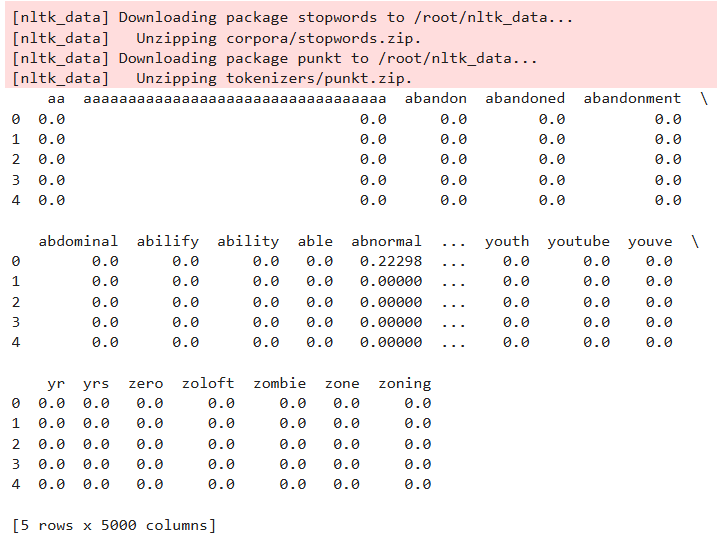
\includegraphics[width=0.8\textwidth]{Images/Output Data Preprocessing.png}  
    \caption{Data Preprocessing}
    \label{Data Preprocessing}  % Label for referencing the figure
\end{figure}

% Bag Of Words Model
\subsubsection{Implementation of Bag Of Words}

\noindent
The following code snippet implements the Bag of Words (BoW) model for the preprocessed dataset related to mental health. This process converts text data into a numerical format that can be used for machine learning tasks.

\begin{verbatim}
import pandas as pd
from sklearn.feature_extraction.text import CountVectorizer
# Load the preprocessed dataset
dataset = pd.read_csv('preprocessed_mental_health_text.csv')
# Check if 'cleaned_text' column exists
if 'cleaned_text' not in dataset.columns:
    raise ValueError("The dataset must have a 'cleaned_text' column. 
    Ensure text preprocessing has been done.")
# Remove rows with missing values in 'cleaned_text' column
dataset.dropna(subset=['cleaned_text'], inplace=True)
# Initialize the CountVectorizer
vectorizer = CountVectorizer()
# Fit and transform the cleaned text data
X = vectorizer.fit_transform(dataset['cleaned_text'])
# Convert the result to a DataFrame for better visualization (optional)
X_df = pd.DataFrame(X.toarray(), columns=vectorizer.
get_feature_names_out())
# Print the shape of the resulting matrix
print(f'Shape of Bag of Words matrix: {X_df.shape}')
# Print the first few rows of the Bag of Words DataFrame (optional)
print(X_df.head())
\end{verbatim}

\noindent
The code begins by importing the necessary libraries: \texttt{pandas} for data manipulation and \texttt{CountVectorizer} from \texttt{sklearn} for creating the Bag of Words model. It then loads a preprocessed dataset from a CSV file named \texttt{preprocessed\_mental\_health\_text.csv}. A check is performed to ensure that the dataset contains a column labeled \texttt{cleaned\_text}. If this column is absent, a \texttt{ValueError} is raised, prompting the user to ensure text preprocessing is completed. Following this, any rows with missing values in the \texttt{cleaned\_text} column are removed to maintain data integrity. Next, an instance of \texttt{CountVectorizer} is initialized, which will convert the cleaned text into a matrix of token counts. The \texttt{fit\_transform()} method is called on the cleaned text data, generating a sparse matrix \(X\) that represents the Bag of Words model. This matrix is then converted into a DataFrame \texttt{X\_df} for easier visualization, with columns corresponding to the unique words identified in the text. Finally, the shape of the resulting Bag of Words matrix is printed to the console, along with the first few rows of the DataFrame to provide a preview of the transformed data.

\begin{figure}[h!]  
    \centering
    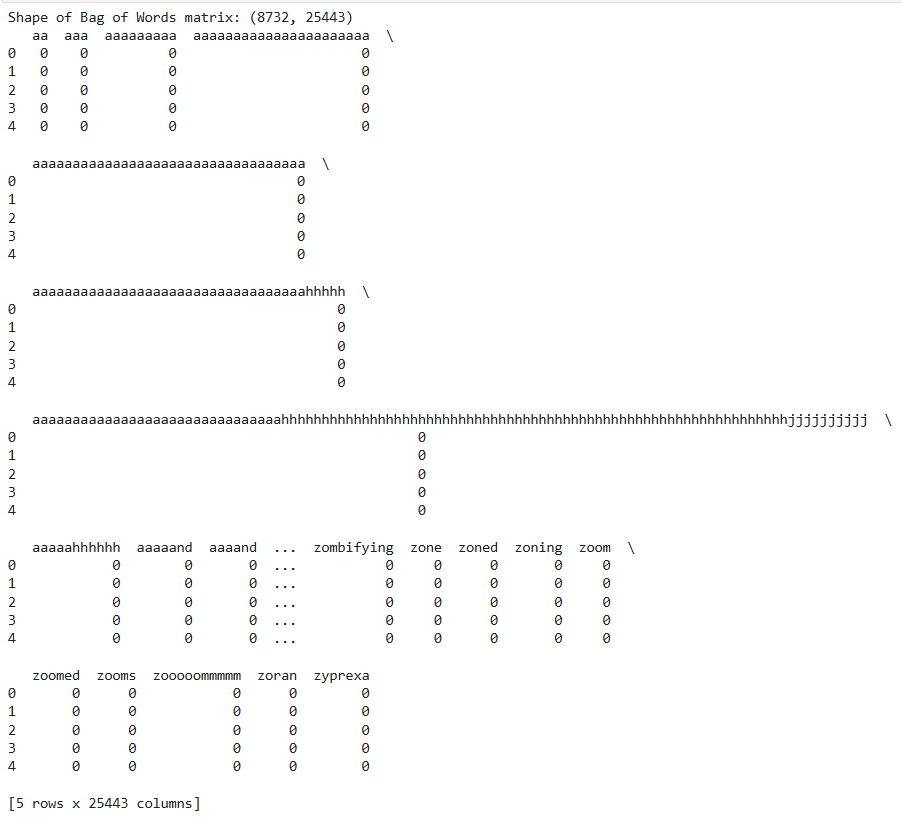
\includegraphics[width=0.8\textwidth]{Images/Output BOW.png}  
    \caption{Implementation of Bag Of Words}
    \label{BOW}  % Label for referencing the figure
\end{figure}

% Splitting DataSet
\subsubsection{Splitting Preprocessed Dataset}
\noindent
The following code snippet demonstrates how to split the preprocessed dataset into training and test sets, which is a crucial step in preparing data for machine learning models.

\begin{verbatim}
import pandas as pd
from sklearn.model_selection import train_test_split

# Load the preprocessed dataset
dataset = pd.read_csv('preprocessed_mental_health_text.csv')

# Check if 'cleaned_text' and 'mental_health_issue' columns exist
if 'cleaned_text' not in dataset.columns or 'mental_health_issue' 
not in dataset.columns:
    raise ValueError("The dataset must have 'cleaned_text' and 
    'mental_health_issue' columns.")

# Remove rows with missing values in 'cleaned_text' column
dataset.dropna(subset=['cleaned_text'], inplace=True) 
#This line has been added

# Initialize the CountVectorizer and fit/transform the cleaned text
from sklearn.feature_extraction.text import CountVectorizer

vectorizer = CountVectorizer()
X = vectorizer.fit_transform(dataset['cleaned_text'])

# Prepare the target variable
y = dataset['mental_health_issue']

# Split the dataset into Training and Test Sets
X_train, X_test, y_train, y_test = train_test_split(X, y, 
test_size=0.2, random_state=42)

# Print the shapes of the resulting datasets
print(f'Shape of X_train: {X_train.shape}')
print(f'Shape of X_test: {X_test.shape}')
print(f'Shape of y_train: {y_train.shape}')
print(f'Shape of y_test: {y_test.shape}')
\end{verbatim}

\noindent
The code begins by importing the necessary libraries, specifically \texttt{pandas} for data manipulation and \texttt{train\_test\_split} from \texttt{sklearn.model\_selection} for splitting the dataset. It then loads 
the preprocessed dataset from a CSV file named \newline
\texttt{preprocessed\_mental\_health\_text.csv}. A validation check is performed to ensure that both the \texttt{cleaned\_text} and 
\texttt{mental\_health\_issue} columns exist in the dataset; if not, a \texttt{ValueError} is raised to alert the user. Next, rows with missing values in the \texttt{cleaned\_text} column are removed to maintain data integrity. After this, the \texttt{CountVectorizer} is initialized to transform the cleaned text into a numerical format suitable for machine learning. The transformed text data is stored in the variable \(X\), while the target variable representing mental health issues is stored in \(y\). The dataset is then split into training and test sets, with 80\% of the data used for training and 20\% for testing, controlled by the \texttt{random\_state} parameter to ensure reproducibility. Finally, the shapes of the resulting training and test datasets are printed to the console, providing insights into the number of samples allocated for training and testing, which is essential for understanding the data distribution.

\begin{figure}[h!]  
    \centering
    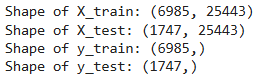
\includegraphics[width=0.6\textwidth]{Images/Output Splitting Dataset.png}  
    \caption{Splitting Dataset}
    \label{Splitting Dataset}  % Label for referencing the figure
\end{figure}


\subsubsection{Logistic Regression}
\noindent
The following code snippet demonstrates the training and evaluation of a Logistic Regression model using a preprocessed dataset related to mental health.

\begin{figure}[h!]  
    \centering
    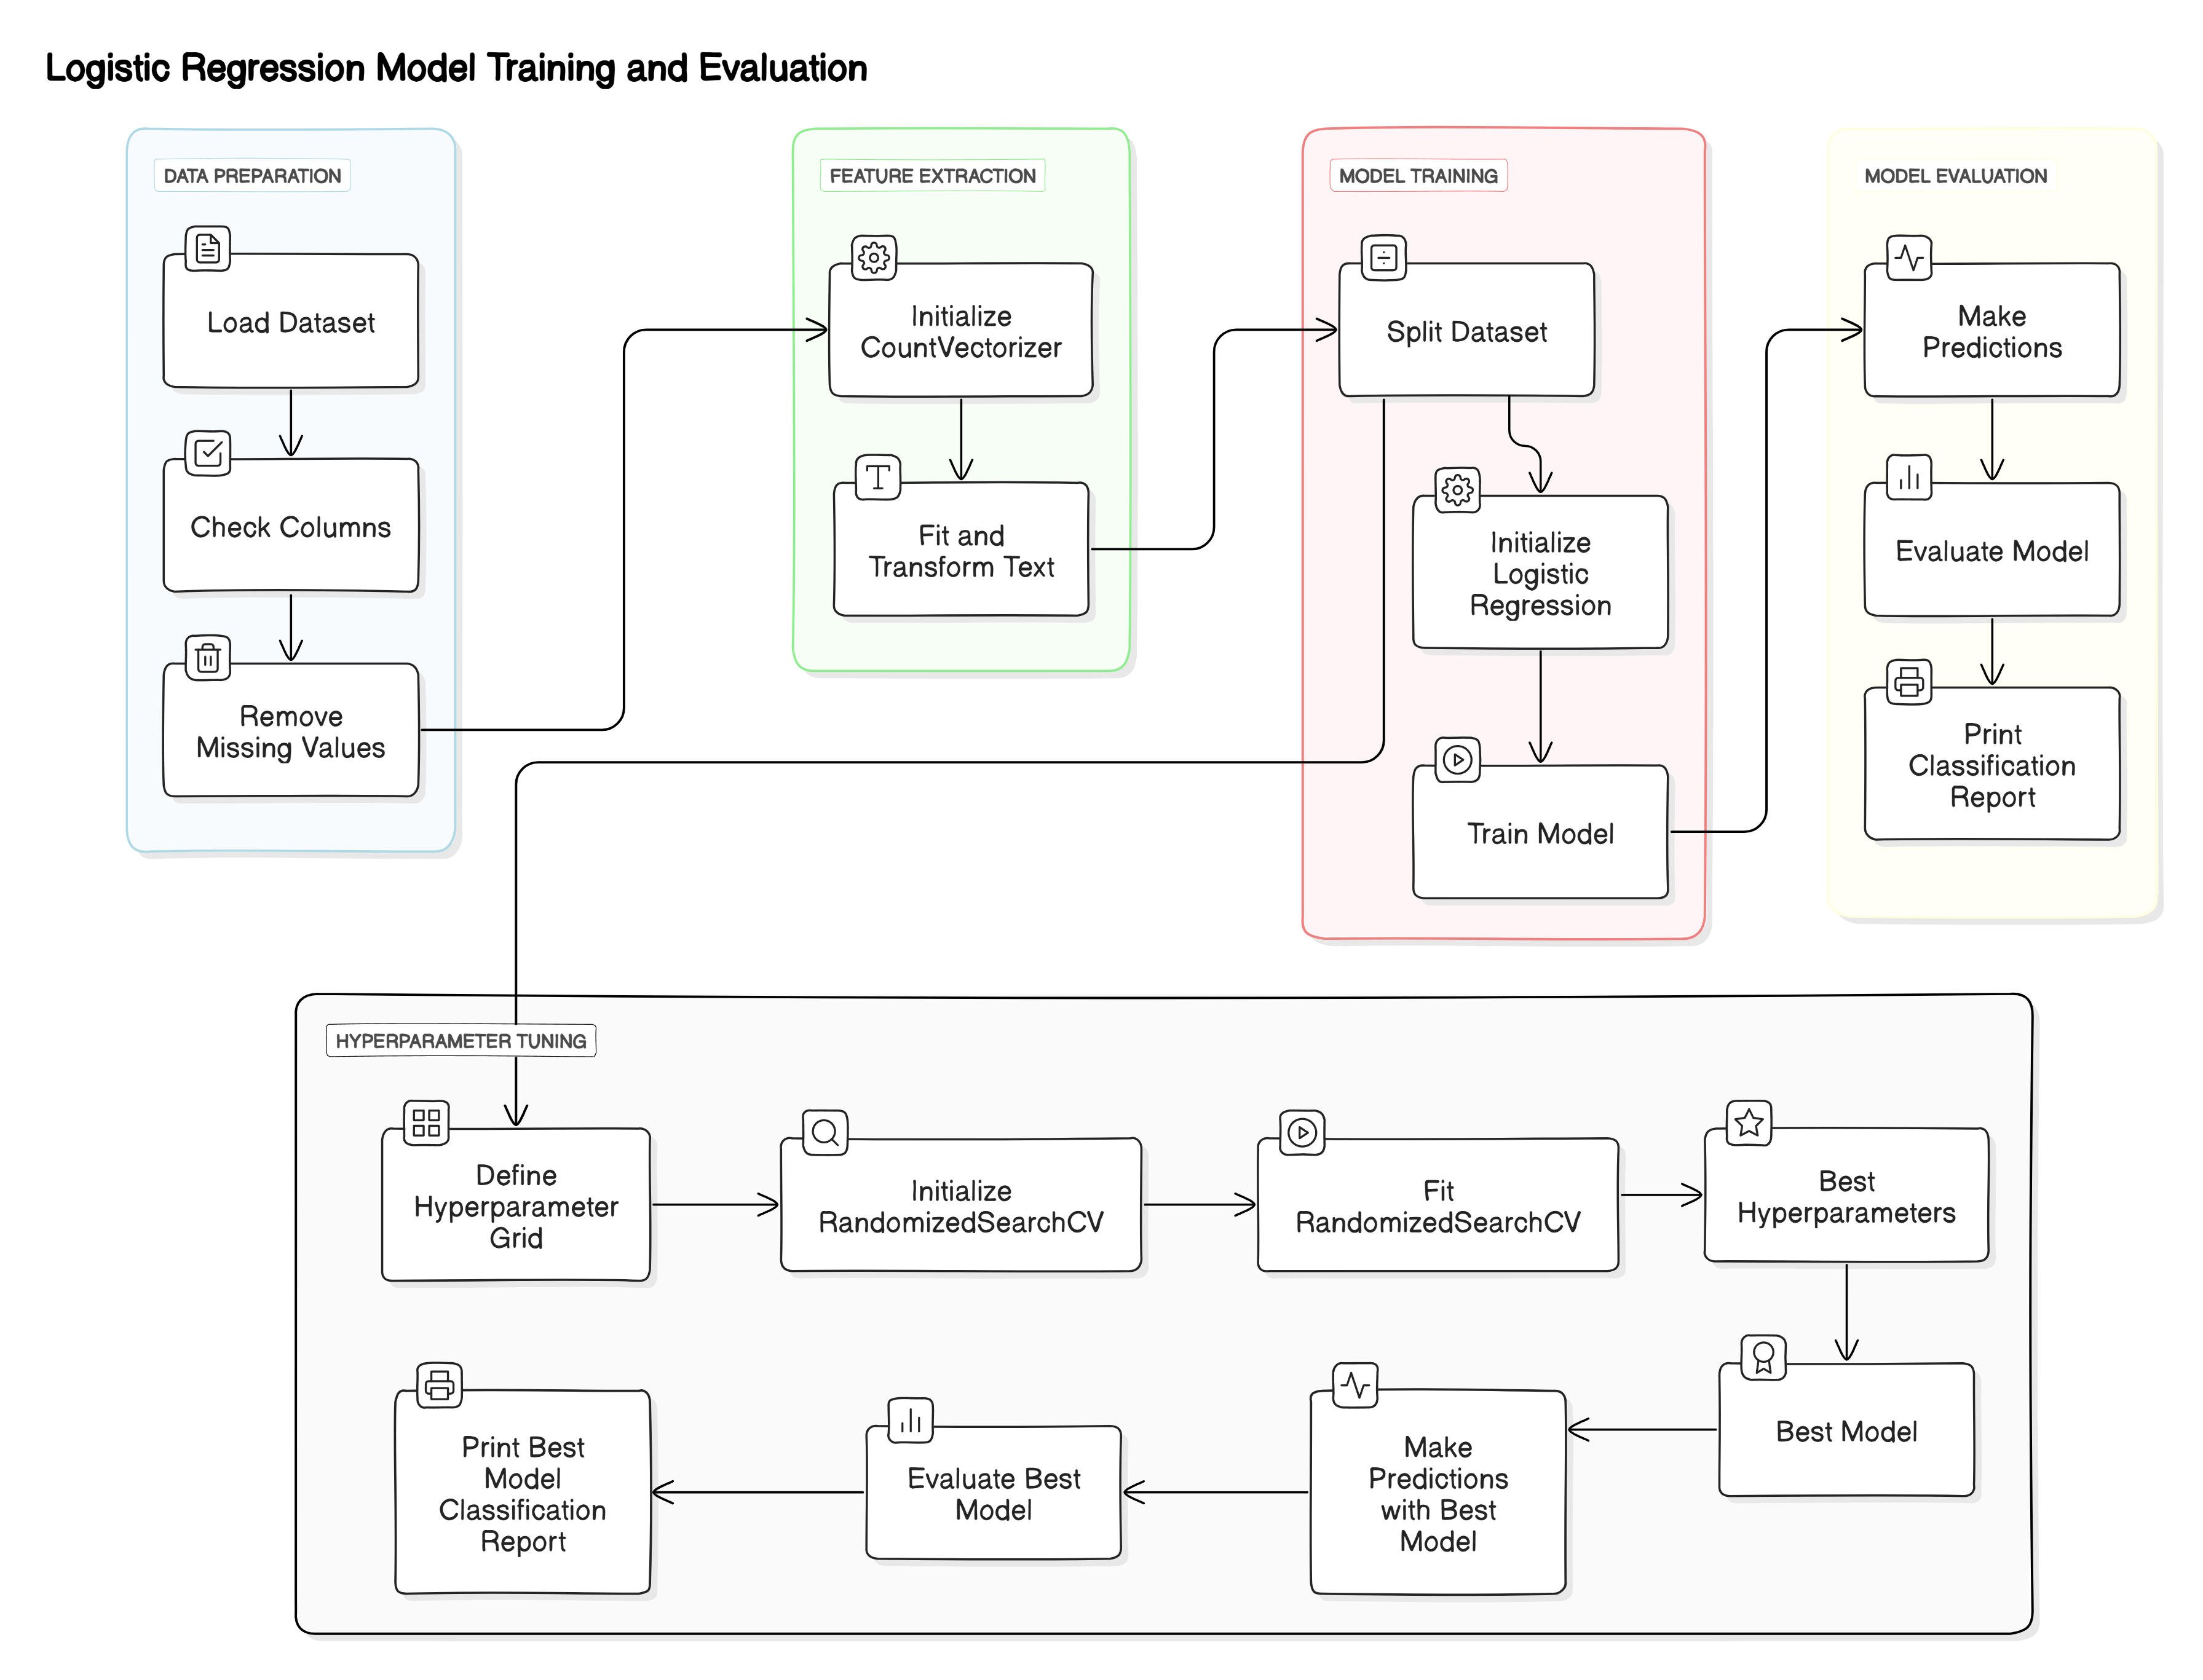
\includegraphics[width=1.0\textwidth]{Images/Logistic Regression.png}  
    \caption{Logistic Regression}
    \label{Logistic Regression}  % Label for referencing the figure
\end{figure}

\begin{verbatim}
import pandas as pd
from sklearn.model_selection import train_test_split
from sklearn.feature_extraction.text import CountVectorizer
from sklearn.linear_model import LogisticRegression
from sklearn.metrics import accuracy_score, classification_report
dataset = pd.read_csv('preprocessed_mental_health_text.csv')
if 'cleaned_text' not in dataset.columns or 'mental_health_issue' 
not in dataset.columns:
    raise ValueError("The dataset must have 'cleaned_text' and 
    'mental_health_issue' columns.")
dataset.dropna(subset=['cleaned_text'], inplace=True)
vectorizer = CountVectorizer()
X = vectorizer.fit_transform(dataset['cleaned_text'])
y = dataset['mental_health_issue']
X_train, X_test, y_train, y_test = train_test_split(X, y, 
test_size=0.2, random_state=42)
model = LogisticRegression(max_iter=2000)
model.fit(X_train, y_train)
y_pred = model.predict(X_test)
accuracy = accuracy_score(y_test, y_pred)
print(f'Accuracy: {accuracy * 100:.2f}%')
print("Classification Report:\n", classification_report(y_test, 
y_pred))
\end{verbatim}

\noindent
The code begins by importing necessary libraries, including \texttt{pandas} for data manipulation and various functions from \texttt{sklearn} for model training and evaluation. It then loads the preprocessed dataset from a CSV file named \texttt{preprocessed\_mental\_health\_text.csv}. A validation check ensures that the dataset contains the required columns, raising an error if either \texttt{cleaned\_text} or \texttt{mental\_health\_issue} is missing. Rows with missing values in the \texttt{cleaned\_text} column are removed to maintain data quality. The \texttt{CountVectorizer} is initialized and used to convert the cleaned text data into a matrix of token counts, stored in \(X\). The target variable, representing mental health issues, is assigned to \(y\). The dataset is then split into training and testing sets, with 80\% used for training and 20\% for testing. A Logistic Regression model is initialized and trained on the training data. Predictions are made on the test set, and the model's accuracy is calculated and printed. Finally, a classification report is generated, providing detailed metrics on the model’s performance across different categories.

\begin{figure}[h!]  
    \centering
    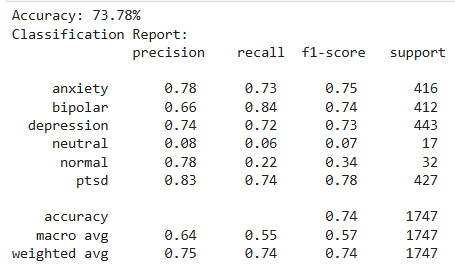
\includegraphics[width=0.8\textwidth]{Images/Output Logistic Regression.png}  
    \caption{Logistic Regression Result}
    \label{Logistic Regression Result}  % Label for referencing the figure
\end{figure}

\subsubsection{Hyperparameter Tuning on Logistic Regression using Random Search}

The following code snippet demonstrates how to perform hyperparameter tuning on a Logistic Regression model using Random Search.

\begin{verbatim}
import pandas as pd
from sklearn.model_selection import train_test_split, 
RandomizedSearchCV
from sklearn.feature_extraction.text import CountVectorizer
from sklearn.linear_model import LogisticRegression
from sklearn.metrics import accuracy_score, classification_report
dataset = pd.read_csv('preprocessed_mental_health_text.csv')
if 'cleaned_text' not in dataset.columns or 'mental_health_issue' 
not in dataset.columns:
    raise ValueError("The dataset must have 'cleaned_text' and 
    'mental_health_issue' columns.")
dataset.dropna(subset=['cleaned_text'], inplace=True)
vectorizer = CountVectorizer()
X = vectorizer.fit_transform(dataset['cleaned_text'])
y = dataset['mental_health_issue']
X_train, X_test, y_train, y_test = train_test_split(X, y, 
test_size=0.2, random_state=42)
model = LogisticRegression(max_iter=200)
param_distributions = {
    'C': [0.001, 0.01, 0.1, 1, 10, 100],
    'penalty': ['l1', 'l2', 'elasticnet', 'none'],
    'solver': ['liblinear', 'saga']
}
random_search = RandomizedSearchCV(estimator=model, 
param_distributions=param_distributions,
n_iter=10, scoring='accuracy', cv=5, n_jobs=-1, random_state=42)
random_search.fit(X_train, y_train)
print("Best Hyperparameters:", random_search.best_params_)
best_model = random_search.best_estimator_
y_pred = best_model.predict(X_test)
accuracy = accuracy_score(y_test, y_pred)
print(f'Accuracy: {accuracy * 100:.2f}%')
print("Classification Report:\n", 
classification_report(y_test, y_pred))
\end{verbatim}

\noindent
The code begins by importing the necessary libraries, including \texttt{pandas} for data manipulation and various functions from \texttt{sklearn} for model training and evaluation. It loads the preprocessed dataset from a CSV file named \newline \texttt{preprocessed\_mental\_health\_text.csv} and checks for the required columns \texttt{cleaned\_text} and \texttt{mental\_health\_issue}. If these columns are not present, a \texttt{ValueError} is raised. The code then removes any rows with missing values in the \texttt{cleaned\_text} column. The \texttt{CountVectorizer} is initialized to convert the cleaned text into a numerical format, which is stored in \(X\), while the target variable representing mental health issues is stored in \(y\). The dataset is split into training and testing sets with 80\% for training and 20\% for testing. A Logistic Regression model is created with a maximum of 200 iterations. The hyperparameter grid for tuning is defined, specifying values for the inverse of regularization strength (\texttt{C}), types of regularization (\texttt{penalty}), and solvers. A \texttt{RandomizedSearchCV} object is initialized to perform the random search over the hyperparameter grid, and the model is fitted using the training data. The best hyperparameters are printed, and the best model is used to make predictions on the test set. Finally, the model's accuracy is calculated and displayed, along with a classification report that provides detailed metrics on the model's performance across different categories.

\begin{figure}[h!]  
    \centering
    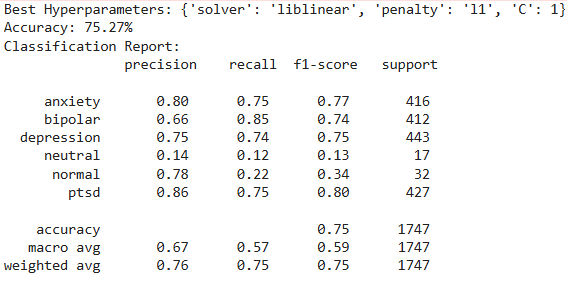
\includegraphics[width=0.6\textwidth]{Images/Output HPT LR.png}  
    \caption{Result of Hyperparameter Tuning on Logistic Regression}
    \label{Project Modules}  % Label for referencing the figure
\end{figure}

\begin{figure}[h!]  
    \centering
    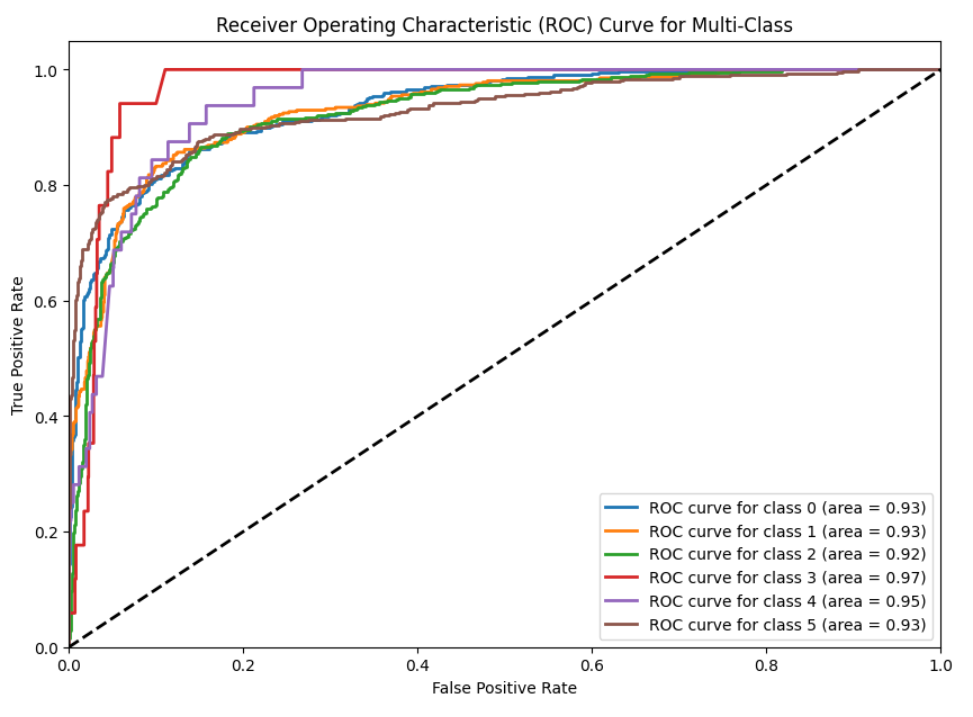
\includegraphics[width=0.6\textwidth]{Images/ROC LR.png}  
    \caption{ROC Curve on Logistic Regression}
    \label{ROC LR}  % Label for referencing the figure
\end{figure}


\subsubsection{K Nearest Neighbours}
\noindent
The following code snippet demonstrates the implementation of the k-Nearest Neighbors (k-NN) algorithm for classifying mental health issues based on preprocessed text data.

\begin{figure}[h!]  
    \centering
    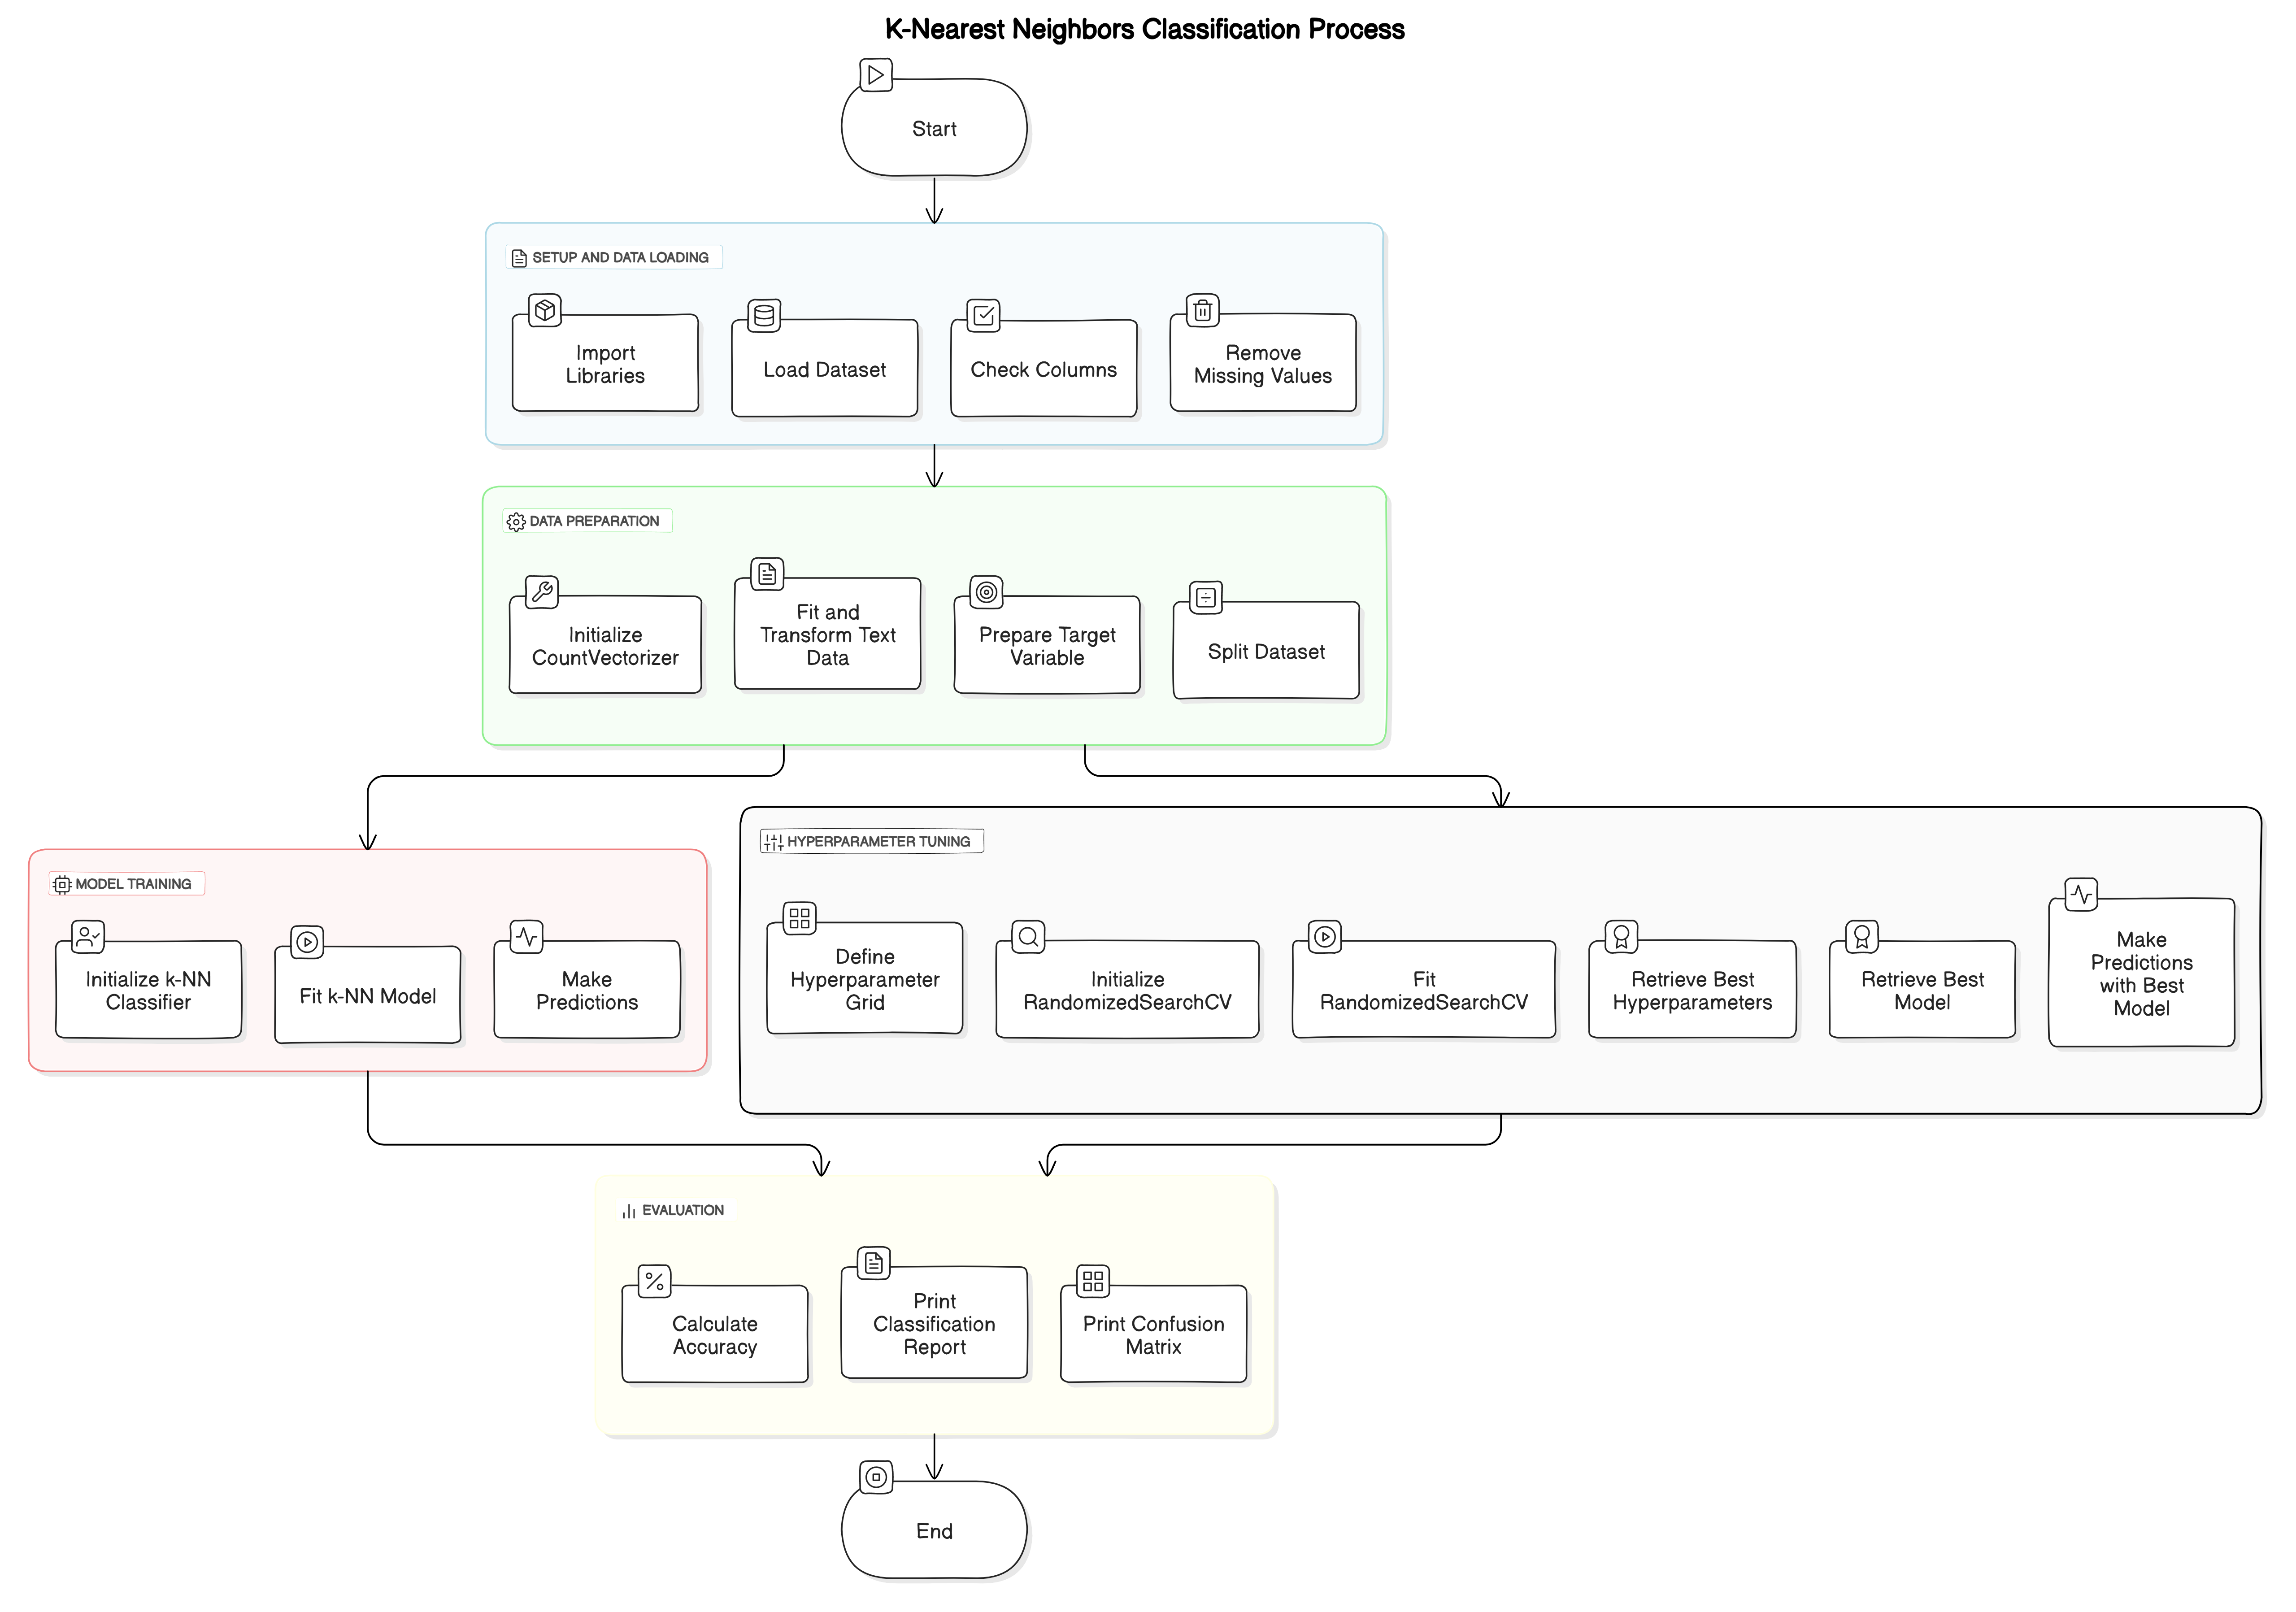
\includegraphics[width=1.0\textwidth]{Images/KNN.png}  
    \caption{K Nearest Neighbours Workflow}
    \label{KNN}  % Label for referencing the figure
\end{figure}


\begin{verbatim}
import pandas as pd
from sklearn.model_selection import train_test_split
from sklearn.feature_extraction.text import CountVectorizer
from sklearn.neighbors import KNeighborsClassifier
from sklearn.metrics import accuracy_score, classification_report, 
confusion_matrix
dataset = pd.read_csv('preprocessed_mental_health_text.csv')
if 'cleaned_text' not in dataset.columns or 'mental_health_issue' 
not in dataset.columns:
    raise ValueError("The dataset must have 'cleaned_text' and 
    'mental_health_issue' columns.")
dataset.dropna(subset=['cleaned_text'], inplace=True)
vectorizer = CountVectorizer()
X = vectorizer.fit_transform(dataset['cleaned_text'])
y = dataset['mental_health_issue']
X_train, X_test, y_train, y_test = train_test_split(X, y, 
test_size=0.2, random_state=42)
knn = KNeighborsClassifier(n_neighbors=5)
knn.fit(X_train, y_train)
y_pred = knn.predict(X_test)
accuracy = accuracy_score(y_test, y_pred)
print(f'Accuracy: {accuracy * 100:.2f}%')
print("Classification Report:\n", 
classification_report(y_test, y_pred))
print("Confusion Matrix:\n", confusion_matrix(y_test,y_pred))
\end{verbatim}

\noindent
The code begins by importing the necessary libraries, including \texttt{pandas} for data manipulation, \texttt{train\_test\_split} for splitting the dataset, \texttt{CountVectorizer} for transforming text data, and \texttt{KNeighborsClassifier} along with various metrics from \texttt{sklearn} for model evaluation. It loads the preprocessed dataset from a CSV file named \newline
\texttt{preprocessed\_mental\_health\_text.csv} and checks that both the \texttt{cleaned\_text} and \texttt{mental\_health\_issue} columns are present; if not, a \texttt{ValueError} is raised. Rows with missing values in the \texttt{cleaned\_text} column are removed to maintain data integrity. The \texttt{CountVectorizer} is initialized to convert the cleaned text into a numerical format, stored in \(X\), while the target variable representing mental health issues is assigned to \(y\). The dataset is split into training and testing sets, with 80\% used for training and 20\% for testing. A k-NN classifier is initialized with 5 neighbors, and the model is fitted on the training data. Predictions are made on the test set, and the model's accuracy is calculated and displayed. Finally, a classification report and confusion matrix are printed, providing detailed metrics on the model's performance and insight into its classification results.

\begin{figure}[h!]  
    \centering
    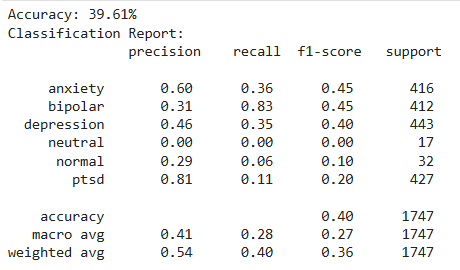
\includegraphics[width=0.6\textwidth]{Images/Output KNN.png}  
    \caption{K Nearest Neighbours Result}
    \label{KNN}  % Label for referencing the figure
\end{figure}

\subsubsection{Hyperparameter Tuning on KNN Using Random Search}
\noindent
The following code snippet demonstrates how to perform hyperparameter tuning on a k-Nearest Neighbors (k-NN) classifier using Random Search to optimize its performance.

\begin{verbatim}
import pandas as pd
from sklearn.model_selection import train_test_split, 
RandomizedSearchCV
from sklearn.feature_extraction.text import CountVectorizer
from sklearn.neighbors import KNeighborsClassifier
from sklearn.metrics import accuracy_score, classification_report, 
confusion_matrix
dataset = pd.read_csv('preprocessed_mental_health_text.csv')
if 'cleaned_text' 
not in dataset.columns or 'mental_health_issue' not in dataset.columns:
    raise ValueError("The dataset must have 'cleaned_text' and 
    'mental_health_issue' columns.")
dataset.dropna(subset=['cleaned_text'], inplace=True)
vectorizer = CountVectorizer()
X = vectorizer.fit_transform(dataset['cleaned_text'])
y = dataset['mental_health_issue']
X_train, X_test, y_train, y_test = train_test_split(X, y, 
test_size=0.2, random_state=42)
knn = KNeighborsClassifier()
param_distributions = {
    'n_neighbors': [3, 4, 5, 6, 7, 8, 9, 10, 11, 12, 13, 
    14, 15, 16, 17, 18, 19, 20],
    'metric': ['euclidean', 'manhattan', 'chebyshev', 'minkowski'],
    'weights': ['uniform', 'distance']
}
random_search = RandomizedSearchCV(estimator=knn, 
param_distributions=param_distributions, 
n_iter=200, scoring='accuracy', cv=5, n_jobs=-1, random_state=42)
random_search.fit(X_train, y_train)
print("Best Hyperparameters:", random_search.best_params_)
best_knn = random_search.best_estimator_
y_pred = best_knn.predict(X_test)
accuracy = accuracy_score(y_test, y_pred)
print(f'Accuracy: {accuracy * 100:.2f}%')
print("Classification Report:\n", 
classification_report(y_test, y_pred))
print("Confusion Matrix:\n", confusion_matrix(y_test, y_pred))
\end{verbatim}

\noindent
The code starts by importing the required libraries, including \texttt{pandas} for data manipulation, and various functions from \texttt{sklearn} for model training, evaluation, and hyperparameter tuning. It loads the preprocessed dataset from a CSV file named \newline \texttt{preprocessed\_mental\_health\_text.csv} and checks for the presence of the necessary columns, raising a \texttt{ValueError} if they are missing. Rows with missing values in the \texttt{cleaned\_text} column are removed to ensure data quality. The \texttt{CountVectorizer} is initialized to convert the cleaned text into a numerical format, stored in \(X\), while the target variable representing mental health issues is assigned to \(y\). The dataset is split into training and testing sets, with 80\% used for training and 20\% for testing. A k-NN classifier is initialized, and a hyperparameter grid is defined, specifying different values for the number of neighbors, distance metrics, and weighting options for the neighbors. The \texttt{RandomizedSearchCV} object is created to perform random search over the hyperparameter grid, and the model is fitted using the training data. After fitting, the best hyperparameters are printed, along with the best k-NN model derived from the search. Predictions are made on the test set, and the accuracy of the model is calculated and displayed. Finally, a classification report and confusion matrix are printed to evaluate the model's performance and provide insights into its classification results.

\begin{figure}[h!]  
    \centering
    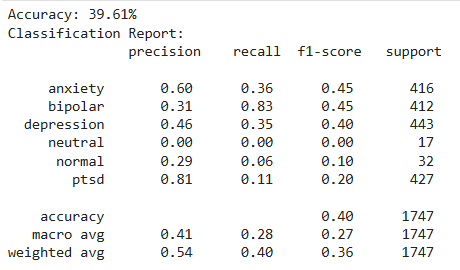
\includegraphics[width=0.8\textwidth]{Images/Output KNN.png}  
    \caption{Result of Hyperparameter Tuning on KNN}
    \label{HPT KNN}  % Label for referencing the figure
\end{figure}

\begin{figure}[h!]  
    \centering
    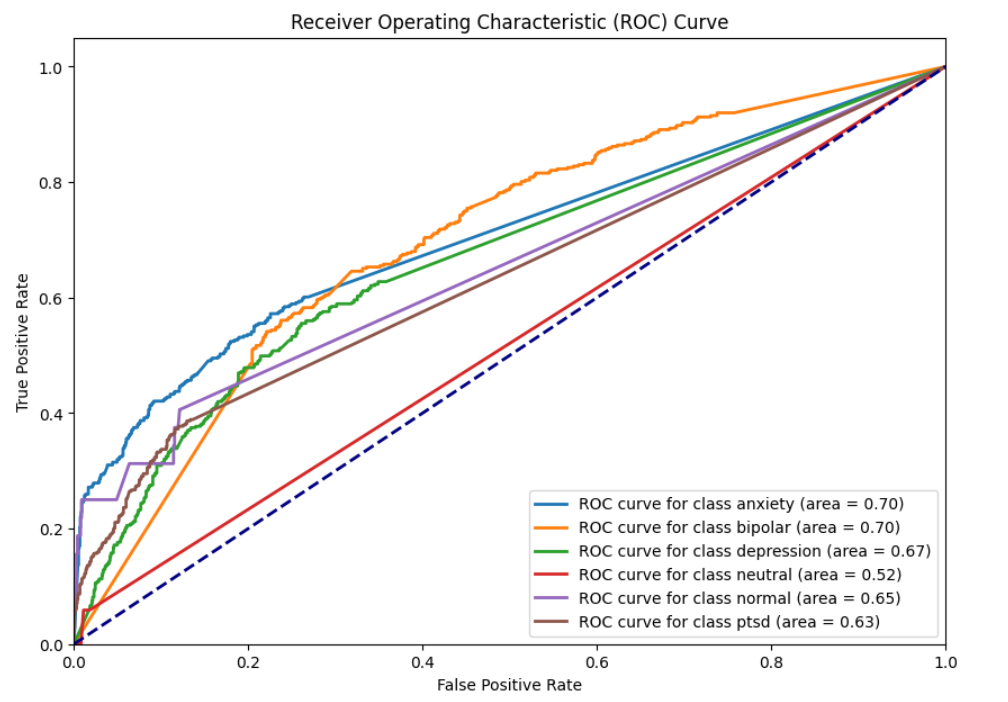
\includegraphics[width=0.8\textwidth]{Images/ROC KNN.png}  
    \caption{ROC curve on KNN}
    \label{ROC KNN}  % Label for referencing the figure
\end{figure}


\subsubsection{Support Vector Machine}
\noindent
The following code snippet demonstrates the implementation of a Support Vector Machine (SVM) classifier for classifying mental health issues based on preprocessed text data.

\begin{figure}[h!]  
    \centering
    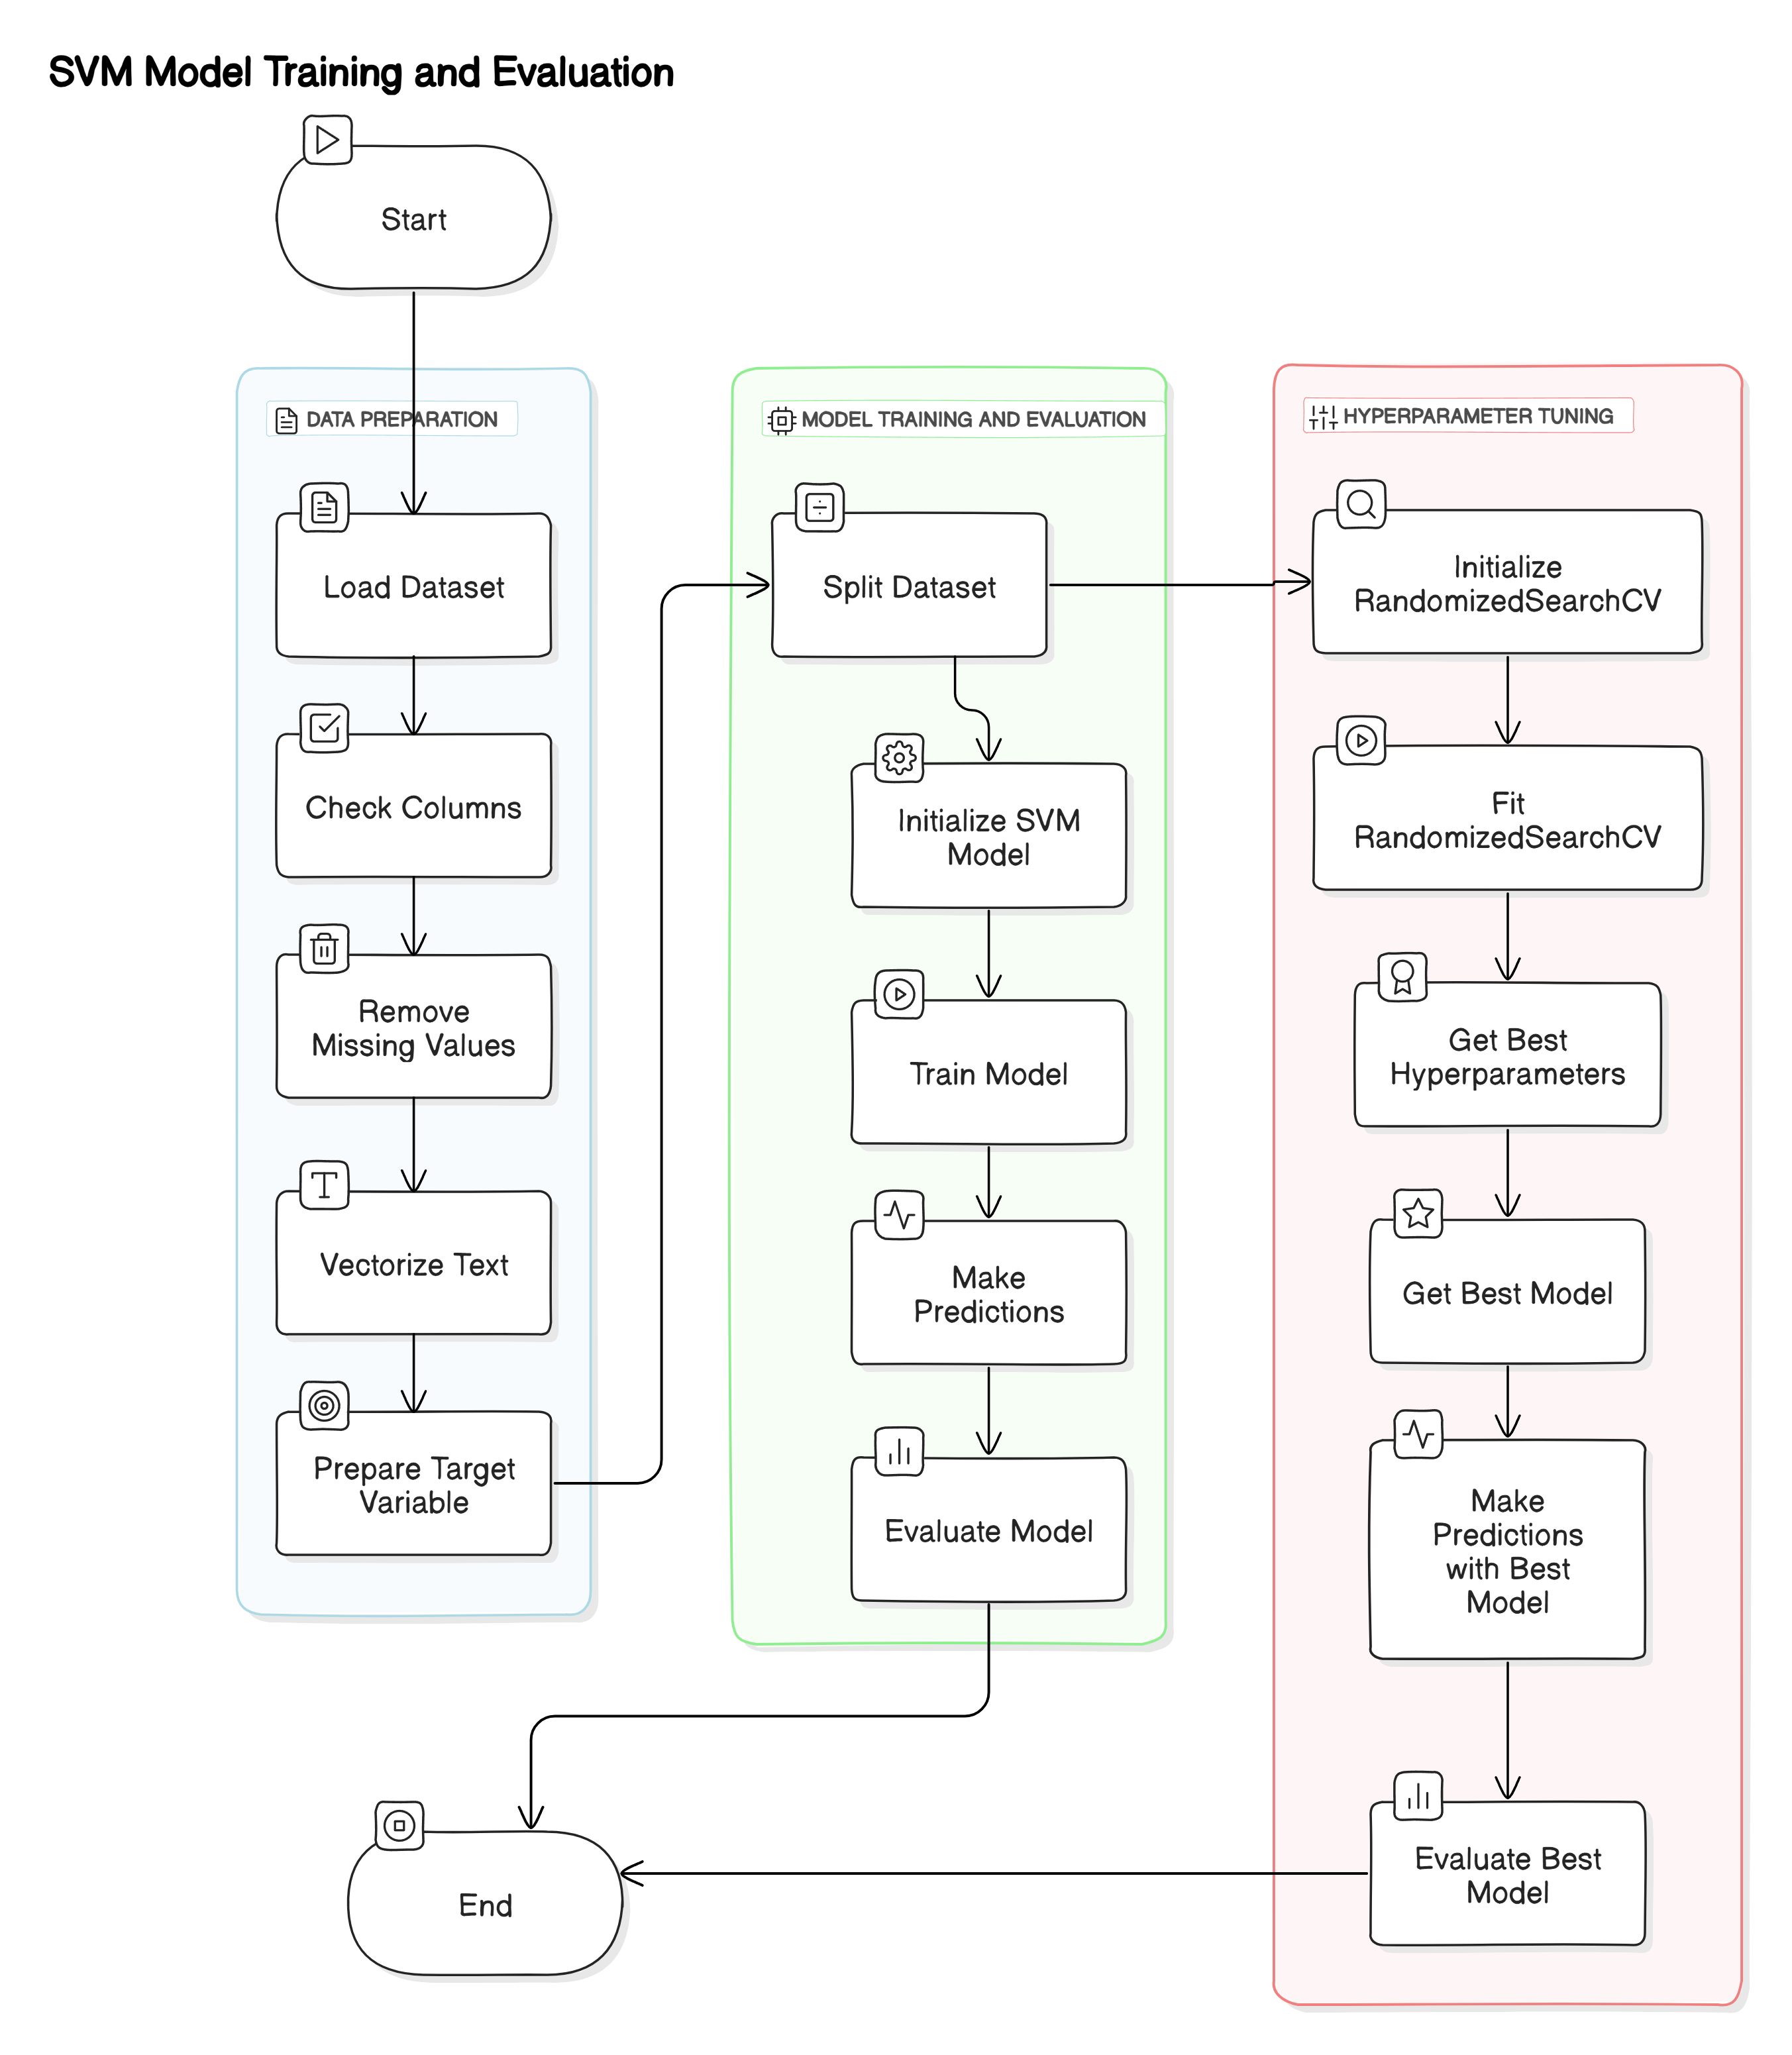
\includegraphics[width=0.6\textwidth]{Images/SVM.png}  
    \caption{Support Vector Machine Workflow}
    \label{SVM}  % Label for referencing the figure
\end{figure}

\begin{verbatim}
import pandas as pd
from sklearn.model_selection import train_test_split
from sklearn.feature_extraction.text import CountVectorizer
from sklearn.svm import SVC
from sklearn.metrics import accuracy_score, classification_report, 
confusion_matrix
dataset = pd.read_csv('preprocessed_mental_health_text.csv')
if 'cleaned_text' not in dataset.columns or 'mental_health_issue' 
not in dataset.columns:
    raise ValueError("The dataset must have 'cleaned_text' and 
    'mental_health_issue' columns.")
dataset.dropna(subset=['cleaned_text'], inplace=True)
vectorizer = CountVectorizer()
X = vectorizer.fit_transform(dataset['cleaned_text'])
y = dataset['mental_health_issue']
X_train, X_test, y_train, y_test = train_test_split(X, y, 
test_size=0.2, random_state=42)
svm_model = SVC(kernel='linear', C=1, random_state=42)
svm_model.fit(X_train, y_train)
y_pred = svm_model.predict(X_test)
accuracy = accuracy_score(y_test, y_pred)
print(f'Accuracy: {accuracy * 100:.2f}%')
print("Classification Report:\n", 
classification_report(y_test, y_pred))
print("Confusion Matrix:\n", confusion_matrix(y_test, y_pred))
\end{verbatim}

\noindent
The code begins by importing the necessary libraries, including \texttt{pandas} for data manipulation and various functions from \texttt{sklearn} for model training and evaluation. It loads the preprocessed dataset from a CSV file named \newline \texttt{preprocessed\_mental\_health\_text.csv} and verifies that both the \texttt{cleaned\_text} and \texttt{mental\_health\_issue} columns exist, raising a \texttt{ValueError} if they are missing. Rows with missing values in the \texttt{cleaned\_text} column are removed to maintain data quality. The \texttt{CountVectorizer} is initialized to convert the cleaned text into a numerical format, stored in \(X\), while the target variable representing mental health issues is assigned to \(y\). The dataset is then split into training and testing sets, with 80\% used for training and 20\% for testing. An SVM model is initialized with a linear kernel and a regularization parameter \(C\) set to 1, which can be adjusted based on the specific needs of the analysis. The model is trained using the training data, and predictions are made on the test set. The accuracy of the model is calculated and displayed, along with a classification report and confusion matrix, which provide insights into the model's performance across different categories and the distribution of classification results.

\begin{figure}[h!]  
    \centering
    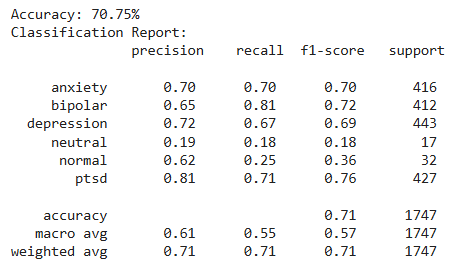
\includegraphics[width=0.6\textwidth]{Images/Output SVM.png}  
    \caption{Support Vector Machine (Linear Kernel) Result}
    \label{SVM}  % Label for referencing the figure
\end{figure}

\subsubsection{Hyperparameter Tuning on SVM using Random Search}
\noindent
The following code snippet demonstrates how to perform hyperparameter tuning on a Support Vector Machine (SVM) classifier using Random Search to optimize its performance.

\begin{verbatim}
import pandas as pd
from sklearn.model_selection import train_test_split, 
RandomizedSearchCV
from sklearn.feature_extraction.text import CountVectorizer
from sklearn.svm import SVC
from sklearn.metrics import accuracy_score, classification_report
dataset = pd.read_csv('preprocessed_mental_health_text.csv')
if 'cleaned_text' not in dataset.columns or 'mental_health_issue'
not in dataset.columns:
    raise ValueError("The dataset must have 'cleaned_text' and 
    'mental_health_issue' columns.")
dataset.dropna(subset=['cleaned_text'], inplace=True)
vectorizer = CountVectorizer()
X = vectorizer.fit_transform(dataset['cleaned_text'])
y = dataset['mental_health_issue']
X_train, X_test, y_train, y_test = train_test_split(X, y, 
test_size=0.2, random_state=42)
model = SVC()
param_distributions = {
    'C': [0.1, 1, 10, 100],
    'kernel': ['linear', 'rbf', 'poly'],
    'gamma': ['scale', 'auto', 0.1, 1],
}
random_search = RandomizedSearchCV(estimator=model, 
param_distributions=param_distributions, 
n_iter=200, scoring='accuracy', 
cv=5, n_jobs=-1, random_state=42)
random_search.fit(X_train, y_train)
print("Best Hyperparameters:", random_search.best_params_)
best_model = random_search.best_estimator_
y_pred = best_model.predict(X_test)
accuracy = accuracy_score(y_test, y_pred)
print(f'Accuracy: {accuracy * 100:.2f}%')
print("Classification Report:\n", 
classification_report(y_test, y_pred))
\end{verbatim}

\noindent
The code begins by importing the required libraries, including \texttt{pandas} for data manipulation and various functions from \texttt{sklearn} for model training and evaluation. It loads the preprocessed dataset from a CSV file named \newline \texttt{preprocessed\_mental\_health\_text.csv} and checks for the necessary columns, raising a \texttt{ValueError} if either the \texttt{cleaned\_text} or \texttt{mental\_health\_issue} columns are missing. Rows with missing values in the \texttt{cleaned\_text} column are then removed to ensure data quality. The \texttt{CountVectorizer} is initialized to convert the cleaned text into a numerical format, stored in \(X\), while the target variable representing mental health issues is assigned to \(y\). The dataset is split into training and testing sets, with 80\% used for training and 20\% for testing. An SVM model is initialized, and a hyperparameter grid is defined that specifies different values for the regularization parameter \(C\), various kernel types, and kernel coefficients. The \texttt{RandomizedSearchCV} object is created to perform random search over the hyperparameter grid, and the model is fitted using the training data. After fitting, the best hyperparameters are printed along with the best SVM model derived from the search. Predictions are made on the test set, and the accuracy of the model is calculated and displayed, along with a classification report that provides detailed metrics on the model's performance.

\begin{figure}[h!]  
    \centering
    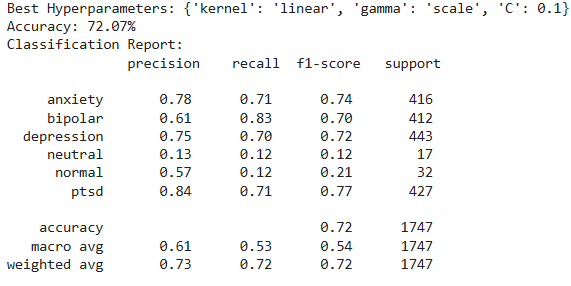
\includegraphics[width=0.8\textwidth]{Images/Output HPT SVM.png}  
    \caption{Result of Hyperparameter Tuning on SVM}
    \label{HPT SVM}  % Label for referencing the figure
\end{figure}

\begin{figure}[h!]  
    \centering
    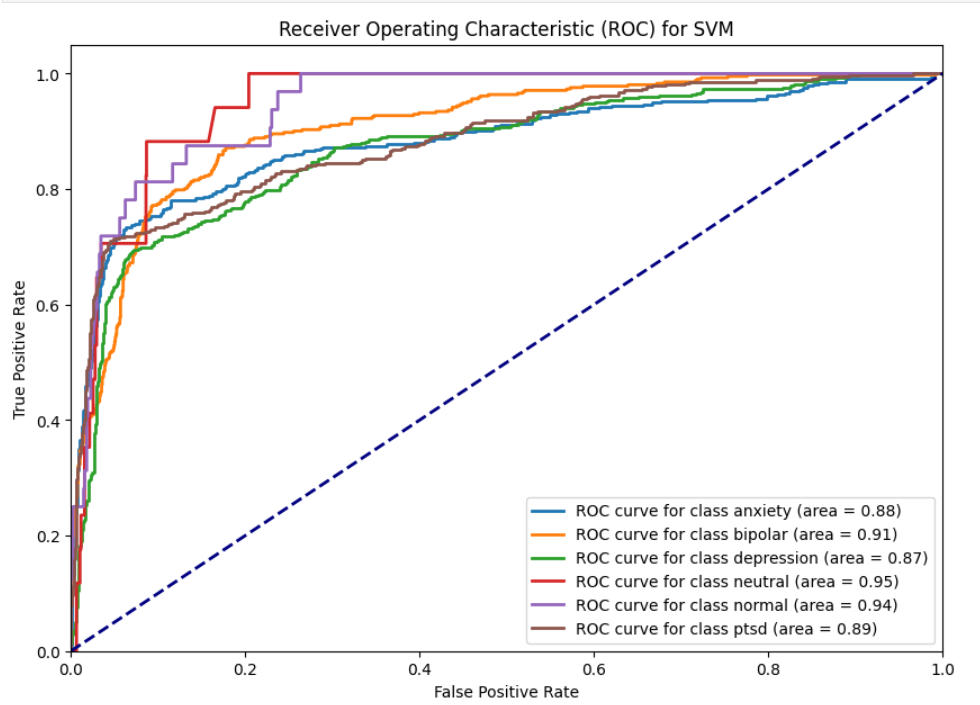
\includegraphics[width=0.8\textwidth]{Images/ROC SVM.png}  
    \caption{ROC Curve on SVM}
    \label{ROC SVM}  % Label for referencing the figure
\end{figure}

\pagebreak

\subsubsection{Naive Bayes Result}
\noindent
The following code snippet demonstrates the implementation of a Naive Bayes classifier for classifying mental health issues based on preprocessed text data.

\begin{figure}[h!]  
    \centering
    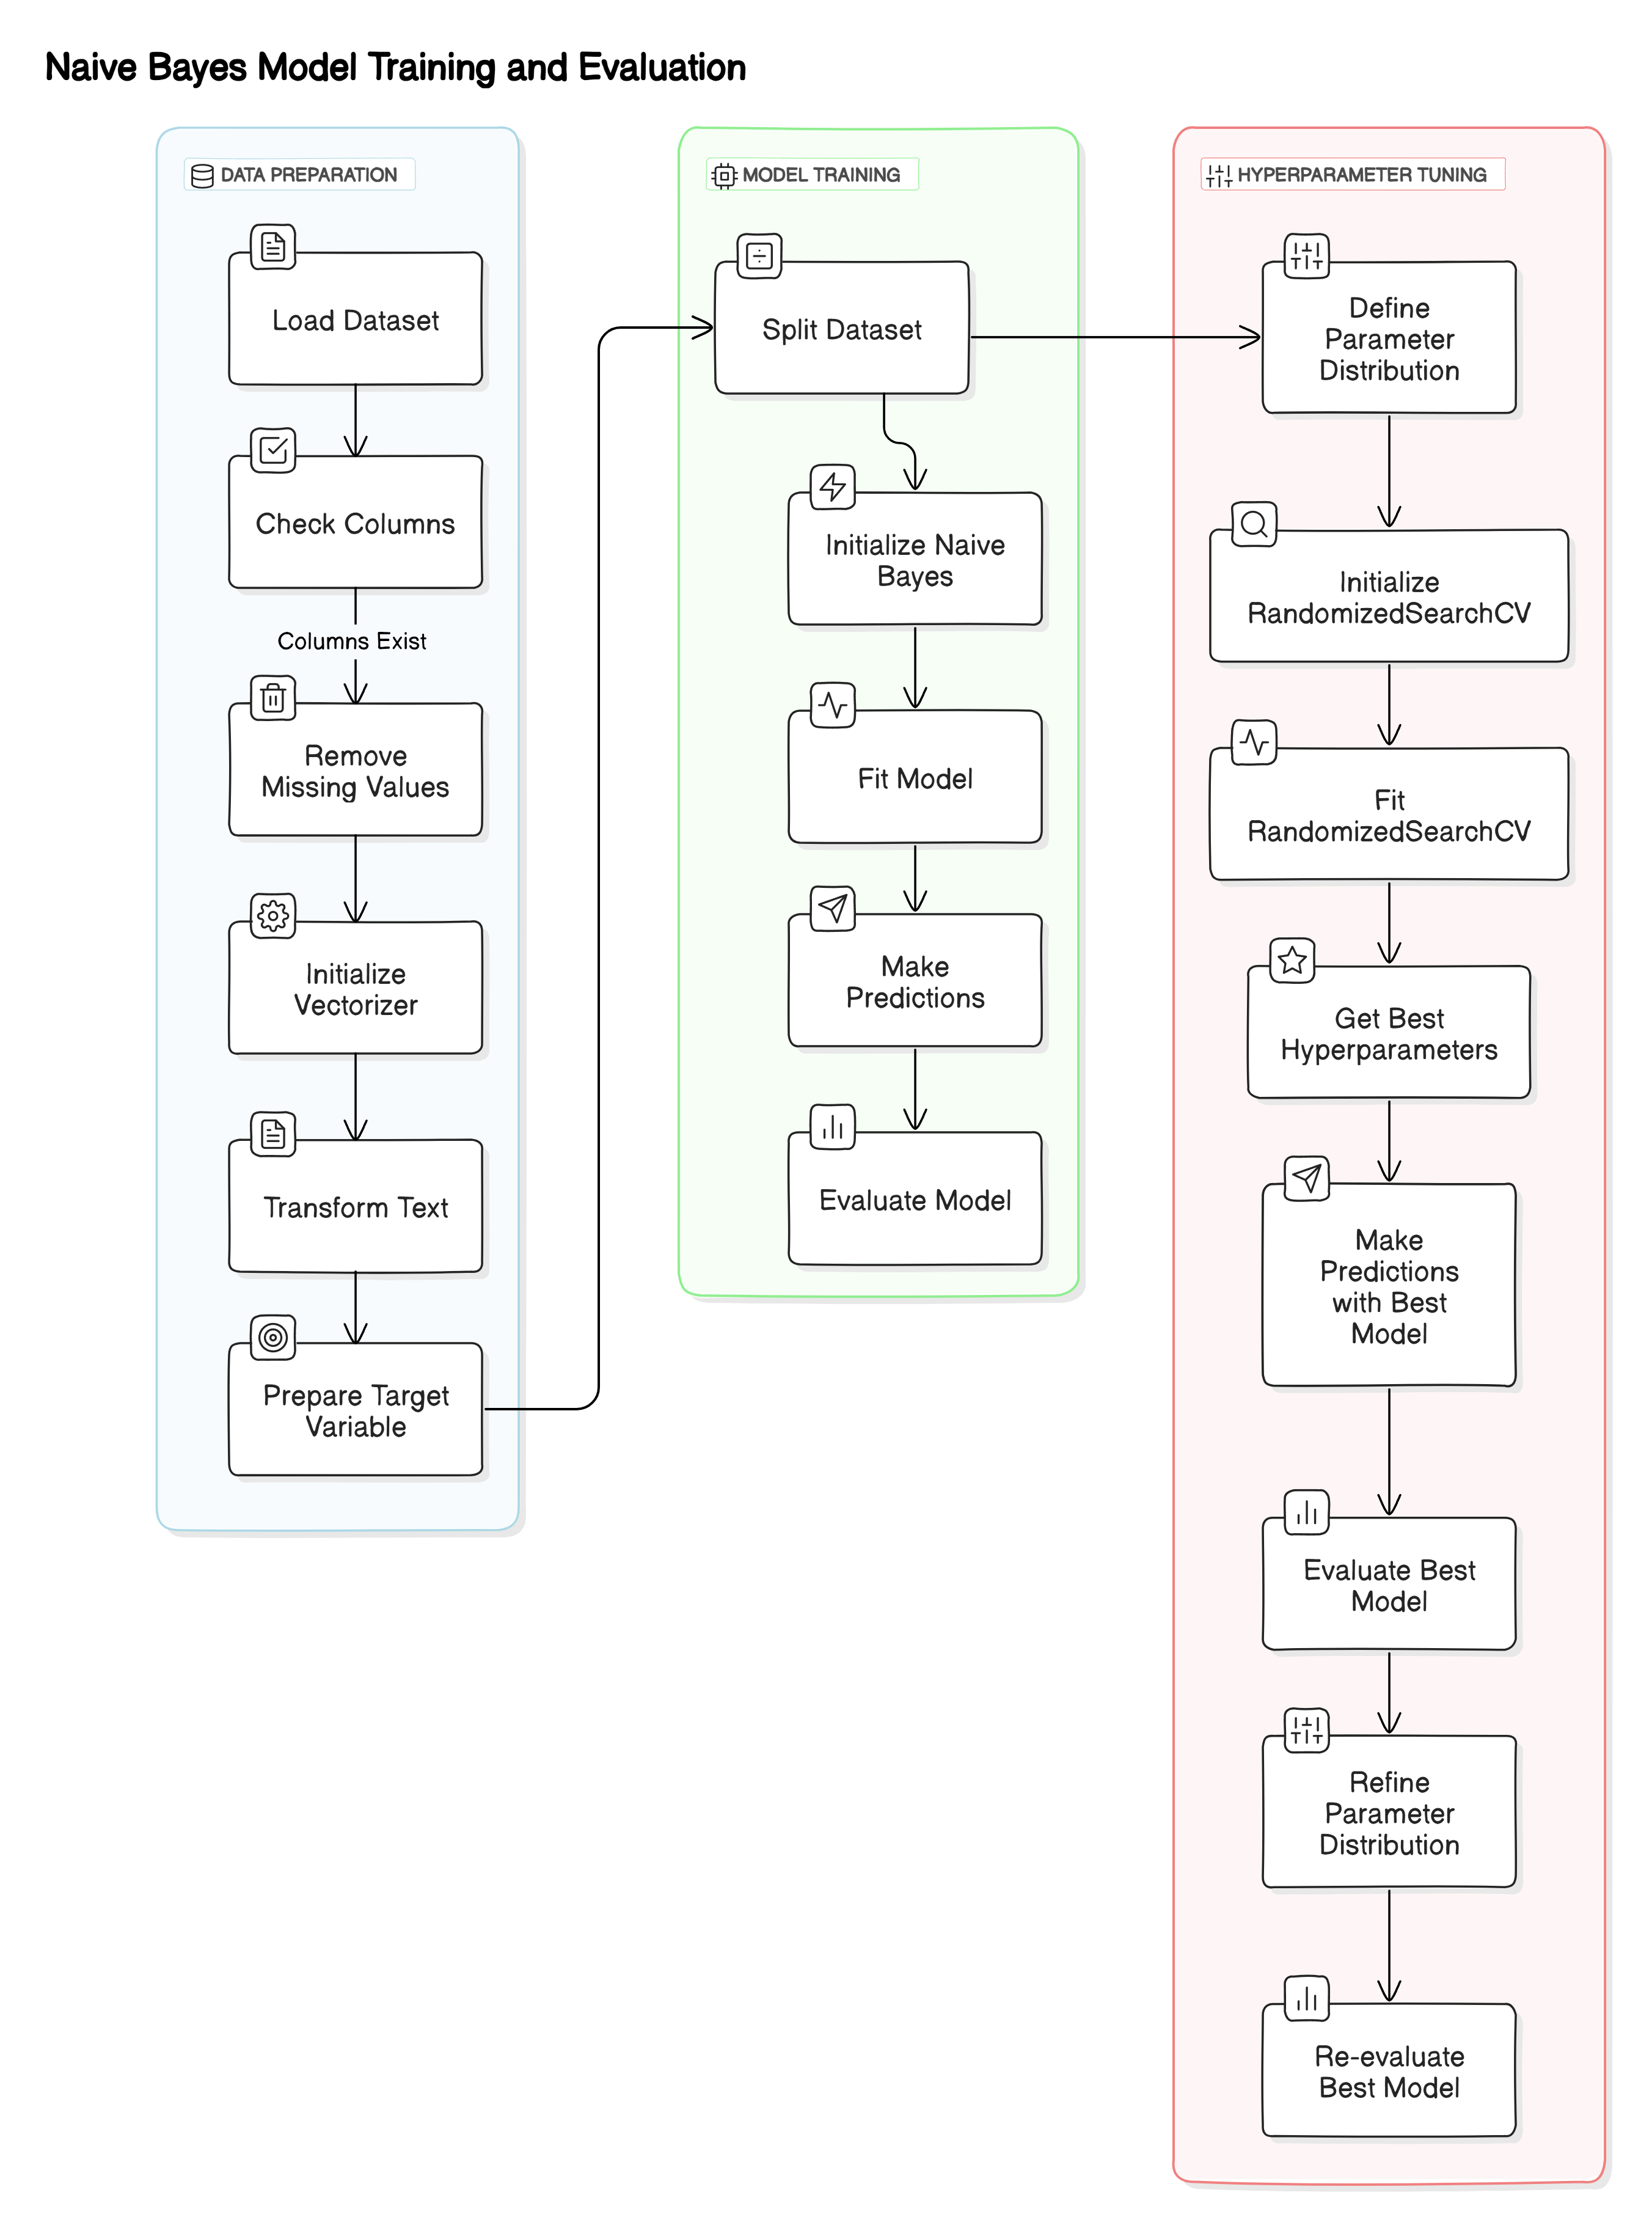
\includegraphics[width=1.0\textwidth]{Images/Naive Bayes.png}  
    \caption{Naive Bayes Workflow}
    \label{Naive Bayes}  % Label for referencing the figure
\end{figure}

\begin{verbatim}
import pandas as pd
from sklearn.model_selection import train_test_split
from sklearn.feature_extraction.text import CountVectorizer
from sklearn.naive_bayes import MultinomialNB
from sklearn.metrics import accuracy_score, classification_report, 
confusion_matrix
dataset = pd.read_csv('preprocessed_mental_health_text.csv')
if 'cleaned_text' not in dataset.columns or 'mental_health_issue' 
not in dataset.columns:
    raise ValueError("The dataset must have 'cleaned_text' and 
    'mental_health_issue' columns.")
dataset.dropna(subset=['cleaned_text'], inplace=True)
vectorizer = CountVectorizer()
X = vectorizer.fit_transform(dataset['cleaned_text'])
y = dataset['mental_health_issue']
X_train, X_test, y_train, y_test = train_test_split(X, y, 
test_size=0.2, random_state=42)
naive_bayes_model = MultinomialNB()
naive_bayes_model.fit(X_train, y_train)
y_pred = naive_bayes_model.predict(X_test)
accuracy = accuracy_score(y_test, y_pred)
print(f'Accuracy: {accuracy * 100:.2f}%')
print("Classification Report:\n", 
classification_report(y_test, y_pred))
print("Confusion Matrix:\n", confusion_matrix(y_test, y_pred))
\end{verbatim}

\noindent
The code begins by importing the necessary libraries, including \texttt{pandas} for data manipulation and various functions from \texttt{sklearn} for model training and evaluation. It loads the preprocessed dataset from a CSV file named \newline
\texttt{preprocessed\_mental\_health\_text.csv} and checks for the required columns, raising a \texttt{ValueError} if either the \texttt{cleaned\_text} or \texttt{mental\_health\_issue} columns are missing. Rows with missing values in the \texttt{cleaned\_text} column are then removed to ensure data quality. The \texttt{CountVectorizer} is initialized to convert the cleaned text into a numerical format, which is stored in \(X\), while the target variable representing mental health issues is assigned to \(y\). The dataset is split into training and testing sets, with 80\% used for training and 20\% for testing. A Naive Bayes classifier, specifically \texttt{MultinomialNB}, is initialized and fitted using the training data. Predictions are made on the test set, and the model's accuracy is calculated and displayed. Finally, a classification report and confusion matrix are printed, providing detailed metrics on the model's performance across different categories and insights into its classification results.

\begin{figure}[h!]  
    \centering
    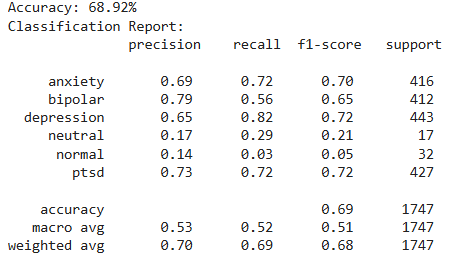
\includegraphics[width=0.8\textwidth]{Images/Output NB.png}  
    \caption{Naive Bayes}
    \label{NB}  % Label for referencing the figure
\end{figure}

\subsubsection{Hyperparameter Tuning on Naive Bayes using Random Search}
\noindent
The following code snippet demonstrates how to perform hyperparameter tuning on a Naive Bayes classifier using Random Search to optimize its performance.

\begin{verbatim}
import pandas as pd
from sklearn.model_selection import train_test_split, 
RandomizedSearchCV
from sklearn.feature_extraction.text import CountVectorizer
from sklearn.naive_bayes import MultinomialNB
from sklearn.metrics import accuracy_score, classification_report, 
confusion_matrix
from scipy.stats import uniform
dataset = pd.read_csv('preprocessed_mental_health_text.csv')
if 'cleaned_text' not in dataset.columns or 'mental_health_issue' 
not in dataset.columns:
    raise ValueError("The dataset must have 'cleaned_text' and 
    'mental_health_issue' columns.")
dataset.dropna(subset=['cleaned_text'], inplace=True)
vectorizer = CountVectorizer()
X = vectorizer.fit_transform(dataset['cleaned_text'])
y = dataset['mental_health_issue']
X_train, X_test, y_train, y_test = train_test_split(X, y, 
test_size=0.2, random_state=42)
naive_bayes_model = MultinomialNB()
param_distributions = {
    'alpha': uniform(0.001, 5.0)
}
random_search = RandomizedSearchCV(estimator=naive_bayes_model, 
param_distributions=param_distributions, n_iter=2000, 
scoring='accuracy', cv=5, n_jobs=-1, random_state=42)
random_search.fit(X_train, y_train)
print("Best Hyperparameters:", random_search.best_params_)
best_model = random_search.best_estimator_
y_pred = best_model.predict(X_test)
accuracy = accuracy_score(y_test, y_pred)
print(f'Accuracy: {accuracy * 100:.2f}%')
print("Classification Report:\n", 
classification_report(y_test, y_pred))
print("Confusion Matrix:\n", confusion_matrix(y_test, y_pred))
\end{verbatim}

\noindent
The code begins by importing the necessary libraries, including \texttt{pandas} for data manipulation, various functions from \texttt{sklearn} for model training and evaluation, and \texttt{uniform} from \texttt{scipy.stats} for sampling. It loads the preprocessed dataset from a CSV file named \texttt{preprocessed\_mental\_health\_text.csv} and checks for the presence of the required columns, raising a \texttt{ValueError} if either the \texttt{cleaned\_text} or \texttt{mental\_health\_issue} columns are missing. Rows with missing values in the \texttt{cleaned\_text} column are removed to maintain data quality. The \texttt{CountVectorizer} is initialized to convert the cleaned text into a numerical format, which is stored in \(X\), while the target variable representing mental health issues is assigned to \(y\). The dataset is split into training and testing sets, with 80\% used for training and 20\% for testing. A Naive Bayes classifier, specifically \texttt{MultinomialNB}, is initialized, and a parameter distribution is defined for hyperparameter tuning using Random Search. The \texttt{RandomizedSearchCV} object is created to perform random search over the hyperparameter grid, and the model is fitted using the training data. After fitting, the best hyperparameters are printed along with the best Naive Bayes model derived from the search. Predictions are made on the test set, and the accuracy of the model is calculated and displayed, along with a classification report and confusion matrix that provide detailed metrics on the model's performance across different categories.

\begin{figure}[h!]  
    \centering
    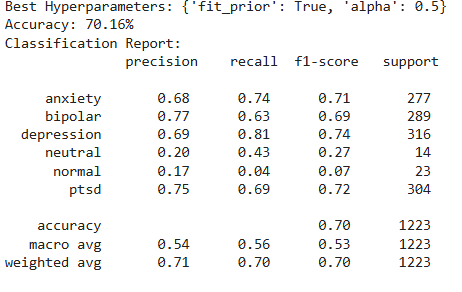
\includegraphics[width=0.8\textwidth]{Images/Output HPT NB.png}  
    \caption{Result of Hyperparameter Tuning on Naive Bayes}
    \label{HPT NB}  % Label for referencing the figure
\end{figure}

\begin{figure}[h!]  
    \centering
    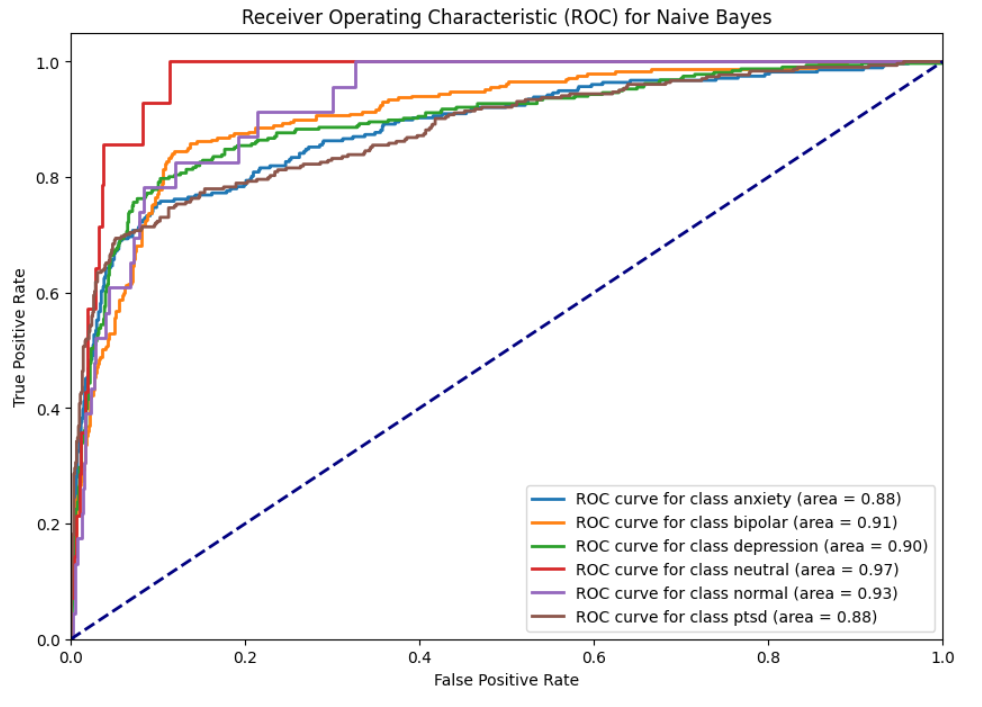
\includegraphics[width=0.8\textwidth]{Images/ROC NB.png}  
    \caption{ROC Curve on Naive bayes}
    \label{ROC NB}  % Label for referencing the figure
\end{figure}


\subsubsection{Random Forest}
\noindent
The following code snippet demonstrates the implementation of a Random Forest classifier for classifying mental health issues based on preprocessed text data.

\begin{figure}[h!]  
    \centering
    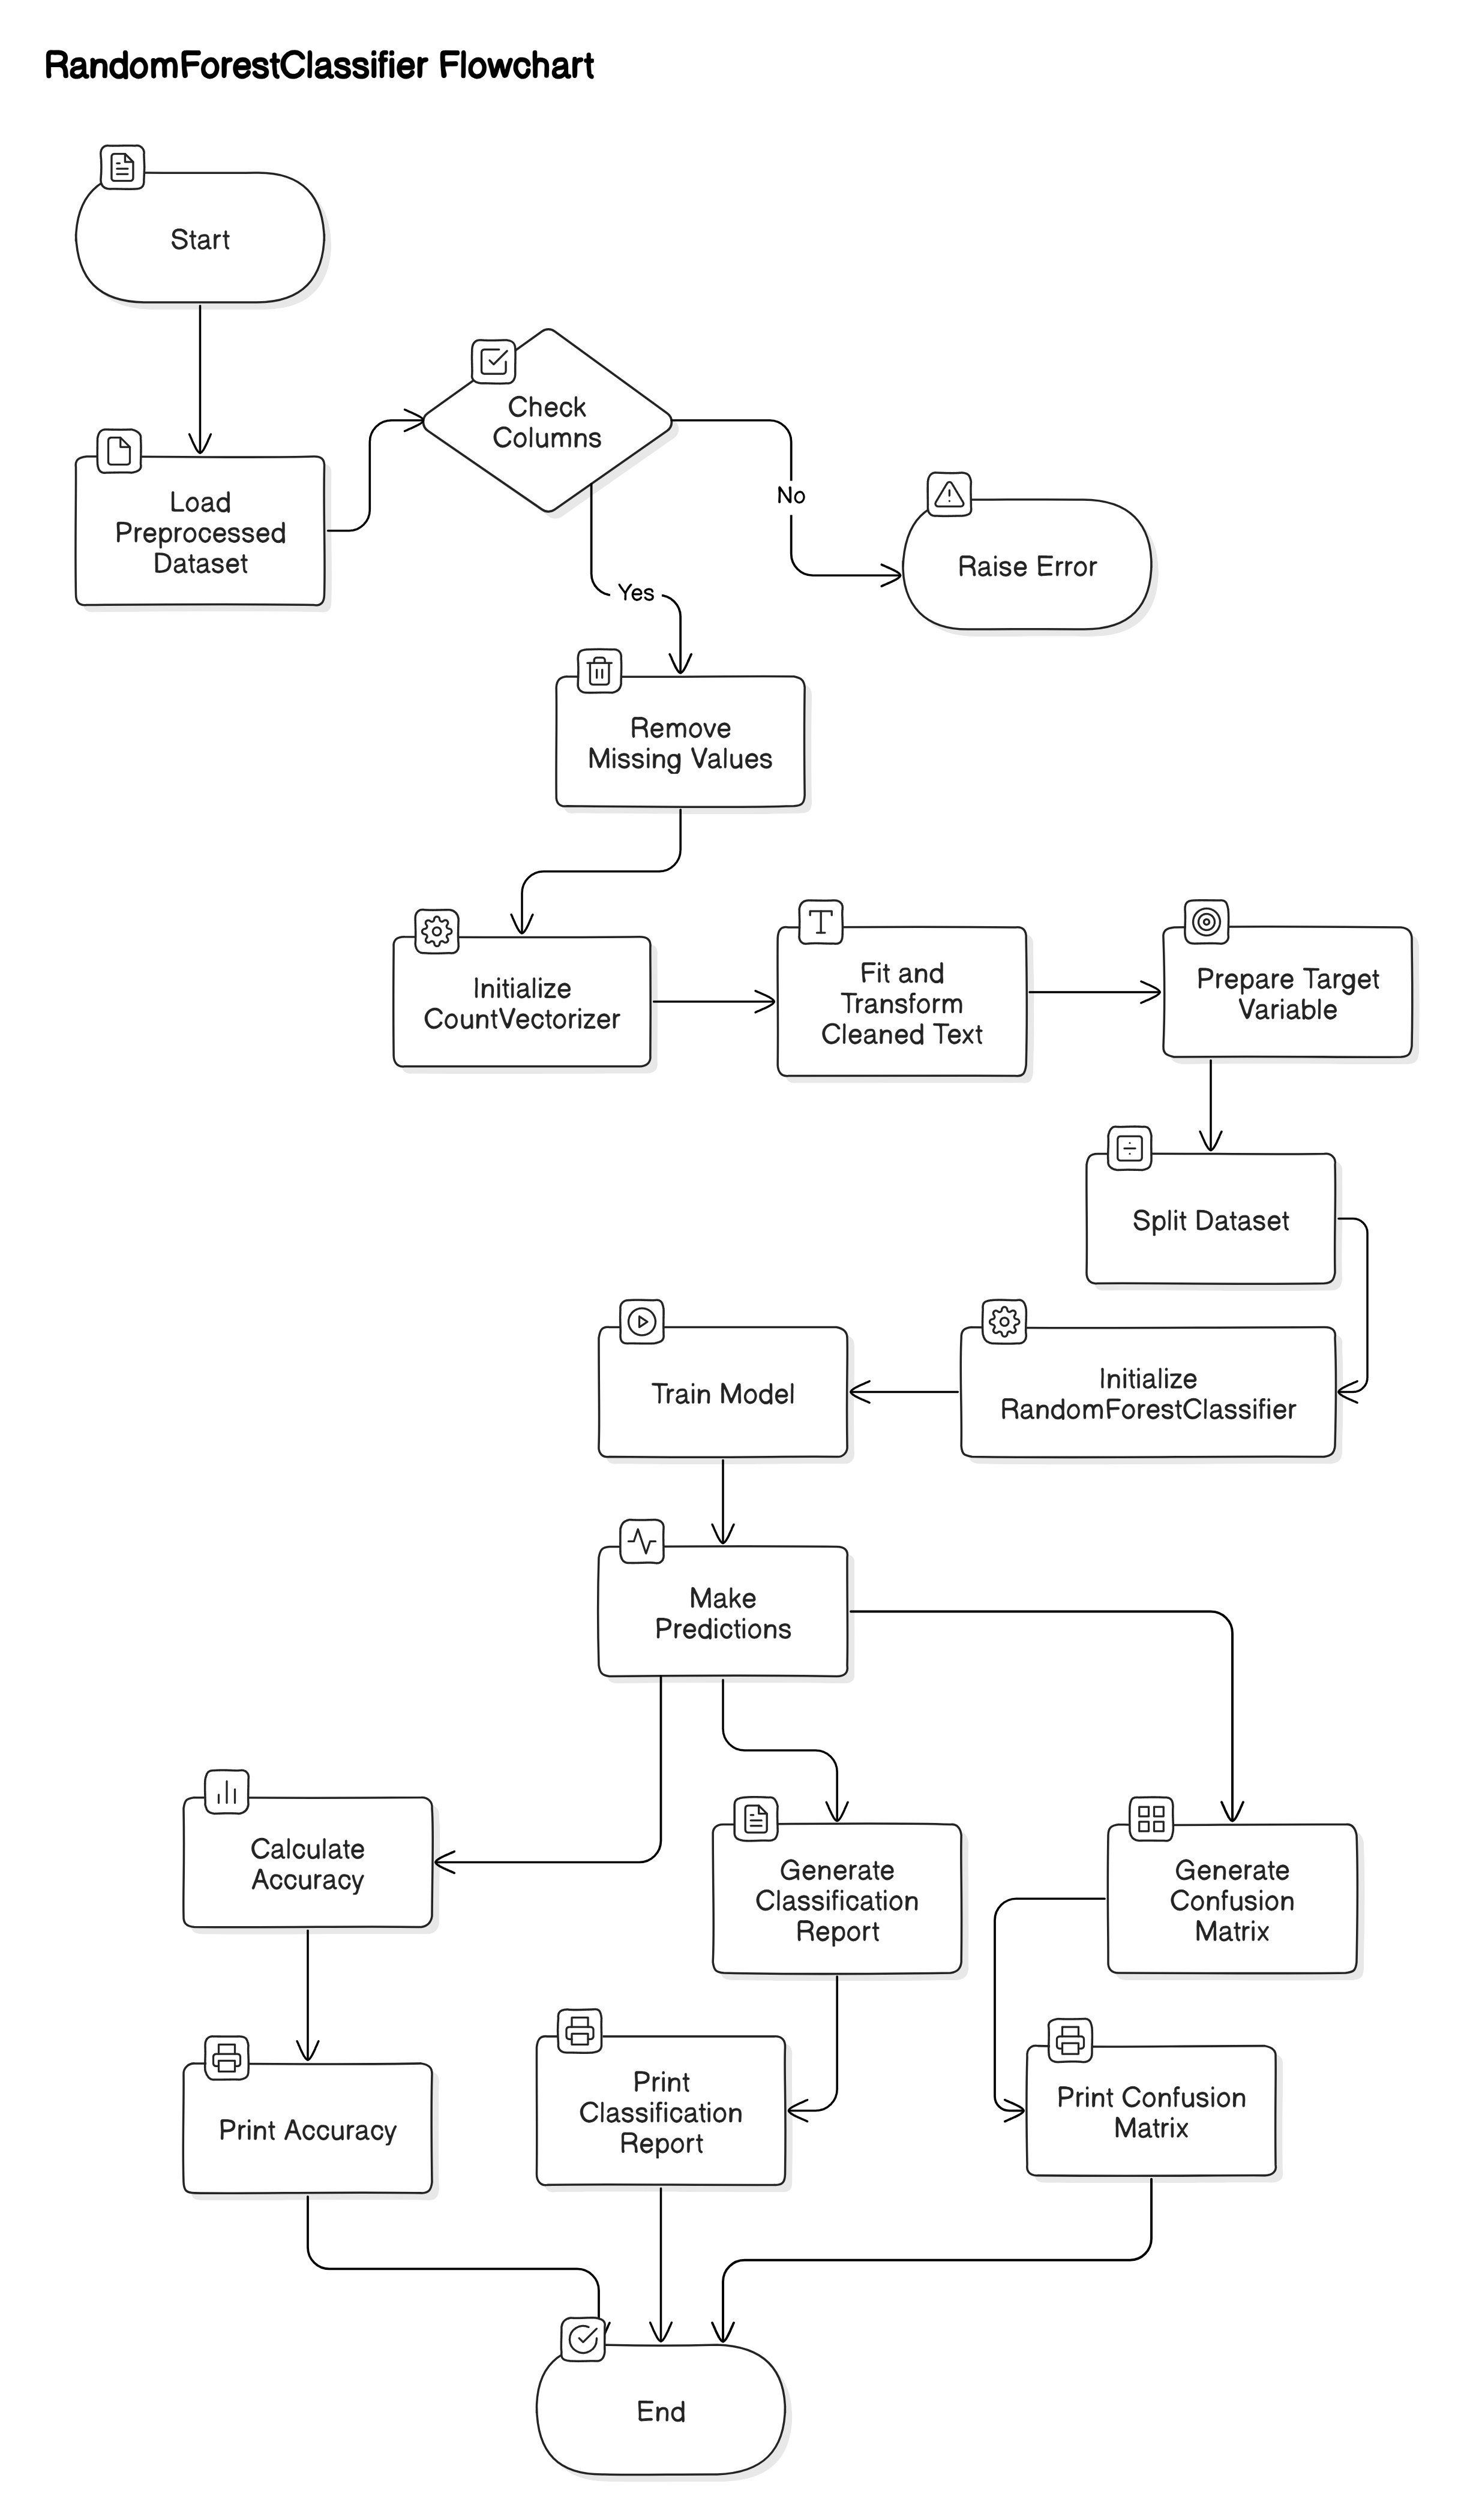
\includegraphics[width=0.6\textwidth]{Images/Random Forest.png}  
    \caption{Random Forest Workflow}
    \label{Random Forest}  % Label for referencing the figure
\end{figure}

\begin{verbatim}
import pandas as pd
from sklearn.model_selection import train_test_split
from sklearn.feature_extraction.text import CountVectorizer
from sklearn.ensemble import RandomForestClassifier
from sklearn.metrics import accuracy_score, classification_report, 
confusion_matrix
dataset = pd.read_csv('preprocessed_mental_health_text.csv')
if 'cleaned_text' not in dataset.columns or 'mental_health_issue' 
not in dataset.columns:
    raise ValueError("The dataset must have 'cleaned_text' and 
    'mental_health_issue' columns.")
dataset.dropna(subset=['cleaned_text'], inplace=True)
vectorizer = CountVectorizer()
X = vectorizer.fit_transform(dataset['cleaned_text'])
y = dataset['mental_health_issue']
X_train, X_test, y_train, y_test = train_test_split(X, y, 
test_size=0.2, random_state=42)
rf_model = RandomForestClassifier(
    n_estimators=3000,
    max_depth=None,
    min_samples_split=20,
    min_samples_leaf=1,
    max_features='sqrt',
    bootstrap=False,
    random_state=42
)
rf_model.fit(X_train, y_train)
y_pred = rf_model.predict(X_test)
accuracy = accuracy_score(y_test, y_pred)
print(f'Accuracy: {accuracy * 100:.2f}%')
print("Classification Report:\n", 
classification_report(y_test, y_pred))
print("Confusion Matrix:\n", confusion_matrix(y_test, y_pred))
\end{verbatim}

\noindent
The code begins by importing the necessary libraries, including \texttt{pandas} for data manipulation and various functions from \texttt{sklearn} for model training and evaluation. It loads the preprocessed dataset from a CSV file named \texttt{preprocessed\_mental\_health\_text.csv} and checks for the presence of the required columns, raising a \texttt{ValueError} if either the \texttt{cleaned\_text} or \texttt{mental\_health\_issue} columns are missing. Rows with missing values in the \texttt{cleaned\_text} column are then removed to ensure data quality. \\

\noindent
The \texttt{CountVectorizer} is initialized to convert the cleaned text into a numerical format, which is stored in \(X\), while the target variable representing mental health issues is assigned to \(y\). The dataset is split into training and testing sets, with 80\% used for training and 20\% for testing. A Random Forest classifier is initialized with specific parameters, including the number of trees (\texttt{n\_estimators}), the minimum number of samples required to split a node (\texttt{min\_samples\_split}), the minimum number of samples in a leaf node (\texttt{min\_samples\_leaf}), and the number of features to consider when looking for the best split (\texttt{max\_features}). The model is then trained using the training data, and predictions are made on the test set. The accuracy of the model is calculated and displayed, along with a classification report and confusion matrix that provide detailed metrics on the model's performance across different categories.

\begin{figure}[h!]  
    \centering
    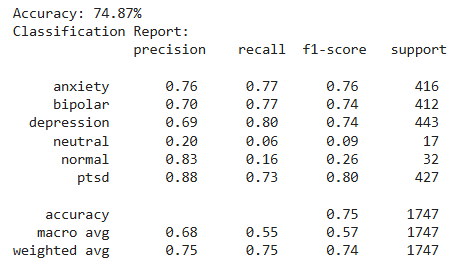
\includegraphics[width=0.9\textwidth]{Images/Output RF.png}  
    \caption{Random Forest Result}
    \label{Random Forest}  % Label for referencing the figure
\end{figure}

\begin{figure}[h!]  
    \centering
    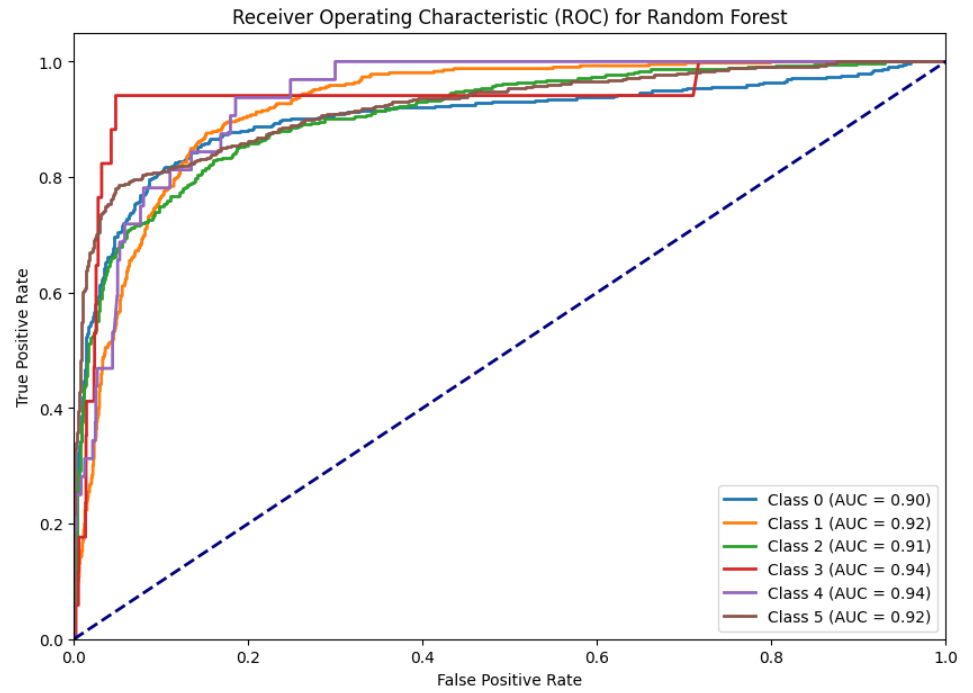
\includegraphics[width=0.9\textwidth]{Images/ROC RF.png}  
    \caption{ROC Curve on Random Forest}
    \label{ROC RF}  % Label for referencing the figure
\end{figure}



% ------------------------- Implementation Ends -----------------------------
